\documentclass[../FinalThesis.tex]{subfiles}
\begin{document}
\chapter{The Effects of Increasing Seasonal Dynamism when Predicting
Connectivity: Advantages or Unnecessary Complications?}
\label{ChapterSeasonality}
\thispagestyle{empty}
\vspace{-1cm}
\noindent\hfil\rule{0.75\textwidth}{.4pt}\hfil

\begin{center}
David D. Hofmann \orcid{0000-0003-3477-4365},
Dominik M. Behr \orcid{0000-0001-7378-8538},
John W. McNutt,
Arpat Ozgul \orcid{0000-0001-7477-2642}, and
Gabriele Cozzi \orcid{0000-0002-1744-1940}

% \begin{flushleft}

% \vspace{5cm}
\vfill

% \textsuperscript{1} Department of Evolutionary Biology and Environmental
% Studies, University of Zurich, Winterthurerstrasse 190, 8057 Zurich,
% Switzerland.
%
% \vspace{0.25cm}
%
% \textsuperscript{2} Botswana Predator Conservation Program, Wild Entrust,
% Private Bag 13, Maun, Botswana.
%
% \vspace{0.25cm}
%
% \textsuperscript{\S} Corresponding author:
% \href{mailto:david.hofmann2@uzh.ch}{david.hofmann2@uzh.ch}

\end{center}

% \vfill

% \textbf{Running Title:} Connectivity in Seasonal Landscapes
%
% \vspace{0.5cm}
%
% \textbf{Keywords:} African wild dog, Connectivity, Dispersal, Dynamism,
% Individual-based, Lycaon pictus, Okavango Delta, Seasonality

% \end{flushleft}

\newpage
\section*{Abstract}

Seasonally changing conditions can drastically alter landscape connectivity.
Nevertheless, most connectivity studies ignore seasonal dynamism and instead
employ a static set of spatial covariates and assume their focal species to
exhibit a static set of preferences. Ignoring seasonality may, however, mask
important ecological features and processes, thus resulting in poor agreement
between predicted and observed movements and therefore a misrepresentation of
connectivity.

We present a simple framework highlighting that seasonality may enter a
connectivity analysis at three distinct stages, namely when (1) extracting
spatial covariates for model fitting, (2) when fitting the selection model, and
(3) when making predictions from the fitted model. In combination, this provides
six possible configurations that differ in terms of the seasonal dynamism they
encapsulate.

Capitalizing on natural seasonal fluctuations of the Okavango Delta in northern
Botswana and on GPS data collected on dispersing African wild dogs
(\textit{Lycaon pictus}) across different seasons, we investigate the degree to
which a better representation of seasonal dynamism improves our ability to
predict dispersal and connectivity. For this, we fit integrated step-selection
functions and predict connectivity using an individual-based dispersal
simulation while explicitly considering seasonal dynamism in both environmental
covariates and the species' preferences.  Using a rigorous cross-validation
procedure, we compare predictive model performances under each of the six
proposed configurations. While we expected that an increasing degree of seasonal
dynamism would lead to improved predictions, we were particularly interested in
identifying at which stage the inclusion of seasonality would provide the
biggest benefits.

We show that, for our study system, improvements in predictive performances
achieved by incorporating seasonal dynamism were moderate. In fact, accounting
for seasonality only improved predictions when an overly simplistic model
formula assumed. Upon using a more complex model formula, the benefits of
accounting for seasonality vanished, resulting in imperceptible performance
differences. Despite this, patterns of connectivity as obtained from dispersal
simulations revealed marked differences between the most static and most dynamic
configurations. Most notably, connectivity was more homogeneously distributed
throughout the study area when seasonality was taken into account, suggesting
the existence of seasonal stepping stones that facilitate dispersal into
otherwise inaccessible areas.

Besides a better understanding of the importance of dynamic connectivity, our
results also provide insights into the conservation needs of the endangered
African wild dog.

\newpage
\section{Introduction}

% \subsection{Connectivity}

Landscape connectivity is defined as the degree to which the landscape
facilitates or impedes movement among habitat patches \citep{Taylor.1993} and is
a central prerequisite for maintaining biodiversity \citep{Fahrig.2003}.
Improved connectivity facilitates dispersal \citep{Doerr.2011, Baguette.2013},
which in turn promotes genetic diversity \citep{Perrin.2000, Frankham.2002} and
the colonization of vacant habitats \citep{Hanski.1999, MacArthur.2001}. Due to
its beneficial impacts on metapopulation dynamics, restoring connectivity is
among the most frequently recommended strategies to conserve biodiversity and to
promote resilience against climate change \citep{Heller.2009, Rudnick.2012}.
Quantifying connectivity and identifying critical dispersal corridors have
therefore become crucial tasks in conservation science \citep{Heller.2009,
Rudnick.2012, Keeley.2019, Hofmann.2021}. One aspect that has received limited
attention in the study of connectivity is the role of seasonality. Yet, seasonal
changes in the environment and an animal's willingness to traverse a particular
habitat type can profoundly impact landscape connectivity \citep{Zeller.2020a}.

% \subsection{Seasonality}

Seasonality can impact functional connectivity through spatio-temporal variation
in the landscape itself, or through temporal variation in species' preferences
towards prevailing conditions \citep{Mui.2017, Simpkins.2017a, Zeller.2020a}. In
ecosystems that experience alternations between wet and dry seasons, for
example, the onset of the rainy season initiates distinct ``green-up'' waves,
which affect the availability of food resources for herbivores and,
subsequently, shape their movements \citep{Merkle.2016}. In its most remarkable
form, the variation in environmental conditions drives herbivore migrations
across massive spatial scales, resulting in short-lived movement corridors
between otherwise disconnected habitats \citep{Serneels.2001, Naidoo.2016}.
Alternatively, seasonality can affect functional connectivity via temporal
changes in a species' habitat preferences. Amphibians, for instance, require
both aquatic and terrestrial habitats, but their preference for one habitat over
the other heavily depends on the season \citep{Baldwin.2006}. Although such
seasonal intricacies are likely to play a fundamental role in many ecosystems,
they only rarely enter connectivity studies in an explicit manner. In fact, most
connectivity studies represent their study system by a static set of
environmental layers and assume that their focal species to exhibit a fixed set
of preferences (e.g., \citealp{Elliot.2014, Abrahms.2017, Brennan.2020}).
However, this may result in biased connectivity estimates and a misallocation of
scarce conservation funds \citep{Osipova.2019, Zeller.2020}. Therefore, a more
dynamic approach to connectivity that acknowledges and renders seasonal
variation has been recommended \citep{Zeller.2020a}.

% \subsection{Modeling Functional Connectivity}

Functional connectivity can be estimated using a variety of modeling techniques
\citep{Diniz.2019}, which all comprise four main steps. First, presence data of
the focal species, preferably collected during dispersal (\citealp{Elliot.2014,
Vasudev.2015, Benz.2016}, but see \citealp{Fattebert.2015}), and a set of
spatial covariate layers that are believed or known to be critical determinants
of connectivity are compiled. Second, these data are combined and fed into a
selection model that enables estimating the focal species' preferences towards
environmental features. Popular frameworks for estimating preferences are
case-control designs, where covariate values extracted at observed locations are
contrasted with those extracted at available locations \citep{Beyer.2010,
Fieberg.2010}. This can be achieved using point-selection functions
\citep{Boyce.2002, Manly.2007}, path-selection functions \citep{Cushman.2010},
and step-selection functions \citep{Fortin.2005, Thurfjell.2014}. A particularly
powerful approach is that of \textit{integrated} step-selection functions
(iSSFs), which provides an effective means to jointly model an animal's movement
kernel (i.e., movement capacity or movement preferences) and habitat-selection
\citep{Avgar.2016, Fieberg.2021}. Third, inferred preferences are used to
predict a permeability surface, which is a spatial layer that indicates the
expected ease or difficulty at which the focal species can traverse a certain
area given the area's environmental characteristics \citep{Zeller.2012}.
Finally, in a fourth step, the permeability surface serves as an input to a
connectivity model that reveals crucial movement corridors. At present, the most
popular connectivity models are least-cost path analysis \citep{Adriaensen.2003}
and circuit theory \citep{McRae.2008}, although individual-based movement models
(IBMMs) have recently gained some momentum too \citep{Kanagaraj.2013,
Allen.2016, Hauenstein.2019, Zeller.2020, UnnithanKumar.2022a,
UnnithanKumar.2022, Hofmann.2023}. A major benefit of using IBMMs is that they
allow estimating connectivity directly via simulated dispersal trajectories,
thus bypassing the generation of a permeability surface
\citep{UnnithanKumar.2022a, Hofmann.2023}.

% \subsection{Incorporating Seasonality in Functional Connectivity Models}

Seasonality can enter the connectivity modeling workflow described above at
three distinct stages (\Cref{GraphicalAbstractCH3}). At the first stage, one can
either extract covariate values on environmental features, such as water and
vegetation, from static layers (i.e., a single snapshot per covariate) or from
stacks of layers (i.e., a sequence of snapshots per covariate) that capture
seasonal variation across the landscape (\Cref{GraphicalAbstractCH3}, Stage 1).
The former approach has historically been the norm (e.g., \citealp{Elliot.2014,
Brennan.2020}), yet advances in remote sensing technologies and a facilitated
access to petabytes of landscape data have opened up new avenues for obtaining
spatial layers at unprecedented spatio-temporal resolutions \citep{Toth.2016,
Rumiano.2020}, such that the representation of study systems via dynamic
covariate layers has become more frequent (e.g., \citealp{Osipova.2019,
Kaszta.2021}). At the second stage, one can assume their focal species to
exhibit a fixed set of preferences across seasons by pooling all presence data,
or can try to account for seasonal changes in preferences by splitting the data
accordingly (\Cref{GraphicalAbstractCH3}, Stage 2; e.g., \citealp{Fortin.2005,
Manly.2007, Cushman.2010, Zeller.2020}). \citet{Chetkiewicz.2009}, for instance,
partitioned their data by season to derive seasonal habitat preferences for
pumas (\textit{Puma concolor}) and grizzlies (\textit{Ursus arctos}). At a third
stage, one can estimate connectivity for either ``average'' environmental
conditions, or utilize seasonally updated layers to estimate connectivity for
distinct seasons (\Cref{GraphicalAbstractCH3}, Stage 3). For connectivity models
that rely on permeability surfaces, the latter case implies repeatedly applying
the connectivity model using seasonally updated permeability surfaces (e.g.
\citealp{Osipova.2019, Zeller.2020, Kaszta.2021, Ciudad.2021}). This is
demonstrated \textit{ad extremum} by \citet{Kaszta.2021}, who prepared monthly
updated permeability surfaces and repeatedly employed circuit theory to estimate
dynamic connectivity for African elephants (\textit{Loxodonta africana}). IBMMs,
by contrast, allow for a more elegant solution, as seasonality can be modeled as
the simulated dispersers move. Such an approach has, however, not yet been
followed. Irrespective of the method used, including seasonality into
connectivity analyses is analytically and computationally demanding
\citep{Bishop-Taylor.2018}, raising the question to what degree it should be
considered.

% \subsection{African wild dogs in Northern Botswana}

To study the importance of seasonal dynamism for dispersal and connectivity, we
use an African wild dog population (\textit{Lycaon pictus}) inhabiting the
seasonally highly variable Okavango Delta ecosystem in northern Botswana as a
study system \citep{McNutt.1996, Wolski.2017}. While once present across the
entire Sub-Saharan continent, the African wild dog has disappeared from a
majority of its historic range due to human persecution, deadly diseases, and
habitat destruction \citep{Woodroffe.2020a}. With about 6,000 adult individuals
remaining in the wild, the species is considered as endangered on the IUCN red
list. Wild dogs are pack-living carnivores, primarily active during the cooler
morning and evening hours \citep{Rasmussen.2012} or during moonlit nights
\citep{Cozzi.2012}. Higher ambient temperature is associated with shorter
activity periods, as the species usually rests during times of elevated heat
\citep{Rabaiotti.2019}. Upon reaching sexual maturity, individuals born into a
pack disperse in single-sex coalitions to find suitable mates and a territory to
settle \citep{McNutt.1996}. In Botswana, the timing of dispersal is seasonal,
with female dispersal peaking prior to the mating season in March, and male
dispersal peaking at the onset of the rainy season in December
\citep{Behr.2020}. Euclidean distances moved by dispersers range from 5 km to
500 km, with some coalitions covering several hundred kilometers within only a
few days \citep{Davies-Mostert.2012, Masenga.2016, Cozzi.2020,
Sandoval-Seres.2022}. Studies of habitat-selection during dispersal show that
wild dogs avoid water, prefer moving along it, prefer moving across open
grassland or shrubs, yet avoid areas dominated by humans and densely covered by
forests \citep{ONeill.2020, Hofmann.2021}. Given the species' considerable
mobility and the study area's significant seasonal variability, we deemed the
study-system well-suited to examine the importance of seasonal dynamism on
dispersal and connectivity.

\begin{figure}[htpb]
 \begin{center}
  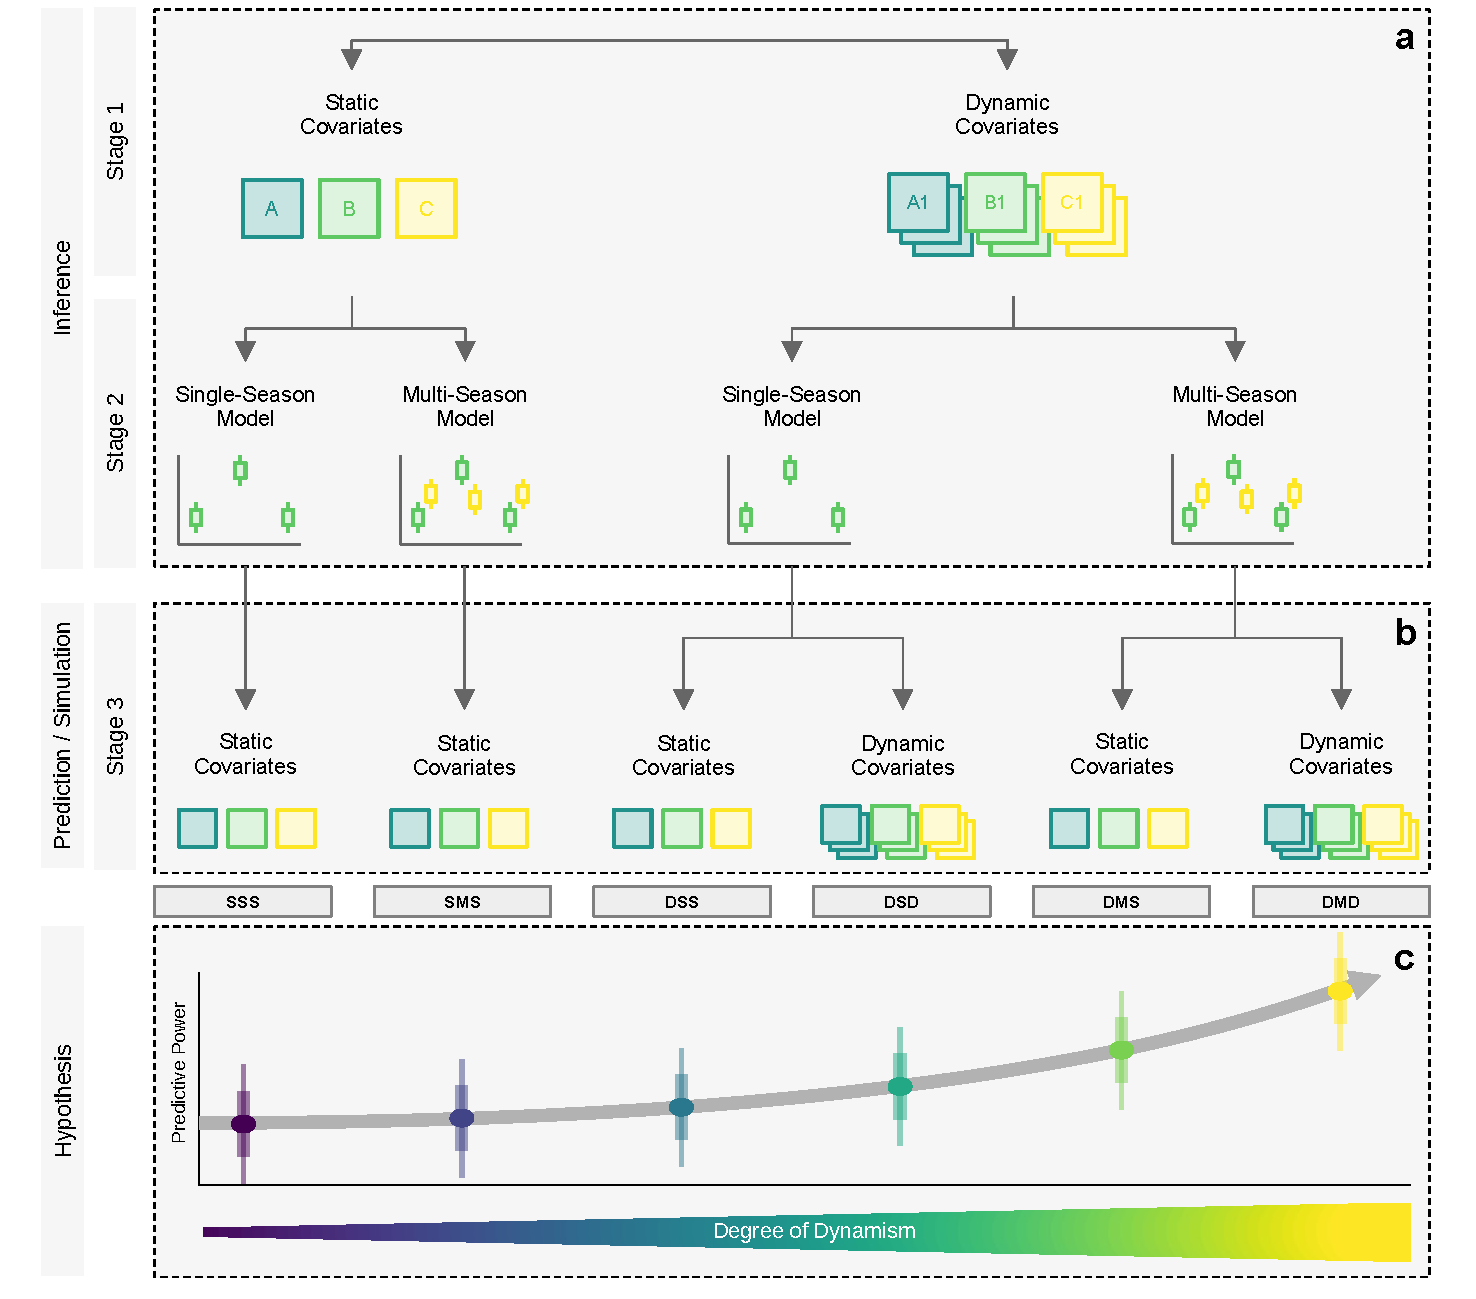
\includegraphics[width = \textwidth]{Figures/GraphicalAbstract.pdf}
  \caption{Overview of the different stages at which seasonality can be rendered
  in studies of dispersal and landscape connectivity. (a) During model fitting,
  one needs to decide whether to represent the environment by a static set of
  covariate layers, thus ignoring seasonality, or to obtain a dynamic set
  covariate layers that allow showing how the landscape changes over time. One
  also needs to decide whether to parameterize a single-season model, assuming
  fixed preferences across the year, or to engage in a multi-season model that
  accounts for seasonal differences. (b) When utilizing the fitted model to
  predict connectivity, one can either assume a static set of environmental
  covariates or again attempt a seasonal take that renders how connectivity
  differs depending on the season. (c) Depending on these decisions, six
  different combinations that differ in terms of the degree of seasonality they
  encapsulate emerge. Our hypothesis was that increasing the degree of dynamism
  when predicting dispersal and connectivity would lead to improved predictions.
  Notably, we were particularly interested in determining at which stage the
  inclusion of seasonally provided the biggest benefits.}
  \label{GraphicalAbstractCH3}
 \end{center}
\end{figure}

Our goal with this article is to (1) create a framework highlighting the
possible avenues through which seasonality can be incorporated into connectivity
analyses, (2) establish whether incorporating seasonality benefits the
predictive performance of dispersal models, and (3) pinpoint at which stages the
inclusion of seasonality provides the largest benefit. For this, we compare the
predictive performances of six configurations that differ in terms of the
dynamism they represent (\Cref{GraphicalAbstractCH3}b). Specifically, we
investigate if and to what degree seasonality at different stages of the
connectivity modeling workflow contributes to improved predictions. We compile
an extensive collection of remote sensed spatial layers that accurately render
seasonality across the Okavango Delta ecosystem. We combine them with multi-year
dispersal data from \inputy{GeneralMetrics/CollarsTotal} dispersing wild dog
coalitions in northern Botswana and apply k-fold cross-validation for
case-control studies to compare the predictive efficacy under each configuration
(\Cref{GraphicalAbstractCH3}b). Finally, we employ IBMMs to simulate dispersal
and estimate connectivity resulting from varying degrees of dynamism. To
distinguish between different configurations, we use codes that highlight the
level of dynamism represented by each configuration (e.g., SSS =
Static-SingleSeason-Static and DMD = Dynamic-MultiSeason-Dynamic). We
hypothesized that habitat-selection and movement behavior of dispersing wild
dogs would differ significantly between seasons and that increasing the degree
of dynamism would result in better agreement between observed and predicted
dispersal patterns (\Cref{GraphicalAbstractCH3}c).

\section{Methods}

We used the \texttt{R} programming language \citep{RCoreTeam.2023} for all data
preparation and analyses. We performed spatial data manipulation using the
\texttt{terra} \citep{Hijmans.2024} and \texttt{spatstat} \citep{Baddeley.2015}
packages. We generated figures using the \texttt{ggplot2} \citep{Wickham.2024}
and \texttt{ggpubr} \citep{Kassambara.2024} packages. To ensure reproducibility
of all our analyses, we provide access to our \texttt{R}-scripts through an
online repository upon publication of this article.

\subsection{Study Area}

The study area comprised the Okavango Delta ecosystem in northern Botswana
(centered at \inputy{GeneralMetrics/StudyAreaCenter.tex} at an elevation of
approx. 950 m) and extended to parts of Namibia and Zimbabwe, encompassing an
extent of \inputy{GeneralMetrics/SizeStudyArea.tex} km\textsuperscript{2}
(\Cref{StudyAreaCH3}). The Okavango Delta is a flood-pulse driven mosaic of
patchy woodlands, permanent swamps, and seasonally flooded grasslands that lie
within the otherwise dry and sandy Kalahari Basin \citep{Wilson.1976,
Ramberg.2006, Mendelsohn.2010}. Precipitation across the study area varies
considerably between seasons, ranging from
\inputy{GeneralMetrics/MinimumPrecipitation.tex} mm during the dry season (from
15 April to 15 October) to \inputy{GeneralMetrics/MaximumPrecipitation.tex} mm
during the wet season (from 15 October to 15 April), totaling to
\inputy{GeneralMetrics/TotalPrecipitation.tex} mm across an average year
(\Cref{Seasonality}a). Daily maximum above-ground temperature fluctuates between
\inputy{GeneralMetrics/MinimumTemperature.tex}\degree C during the dry winter
months and \inputy{GeneralMetrics/MaximumTemperature.tex}\degree C during the
wet summer months (\Cref{Seasonality}b). The vegetation in the study area is
mainly composed of mopane forest (\textit{Colophospermum mopane}), mixed
woodland acacia-dominated (\textit{Acacia spp.}), and grassland. Substantial
vegetation green-up (e.g., plant and shoots growth, leaf production, and grass
greening) after the dry season starts with a delay of some weeks after the onset
of the first rains in the wet season. The normalized difference vegetation index
(NDVI) therefore depicts a smoothed and lagged response to precipitation
patterns across the study area (\Cref{Seasonality}c). The yearly flood-cycle of
the Okavango Delta is predominantly driven by rainfalls in the Angolan
highlands, where water is collected and channeled through the Cubango and Cuito
rivers into the Okavango Delta \citep{McCarthy.2003, Gumbricht.2004,
Mendelsohn.2010}. Because water only slowly descends from the catchment areas in
Angola into the Delta's tributaries, the flood is out of sync with local
rainfalls and reaches its maximum extent during August-September, i.e. during
peak dry season (\citealp{Wolski.2017}, \Cref{Seasonality}d). While the extent
of large-bodied rivers and floodplains is determined by precipitation in Angola,
the emergence of smaller, ephemeral water-bodies (i.e., pans) is dictated by
local precipitation during the wet season.
\inputy{GeneralMetrics/PercentageProtected.tex}\% of the landscape in the study
area form part of a protected area, such that human impact remains low and
largely limited to settlements along the western part of the Okavango Delta and
the city of Maun at the Delta's southern tip (\Cref{StudyAreaCH3}). Landscapes
outside protected areas in Zimbabwe, however, are more heavily influenced by
humans, mainly through agricultural fields and human settlements.

\begin{figure}[htpb]
 \begin{center}
  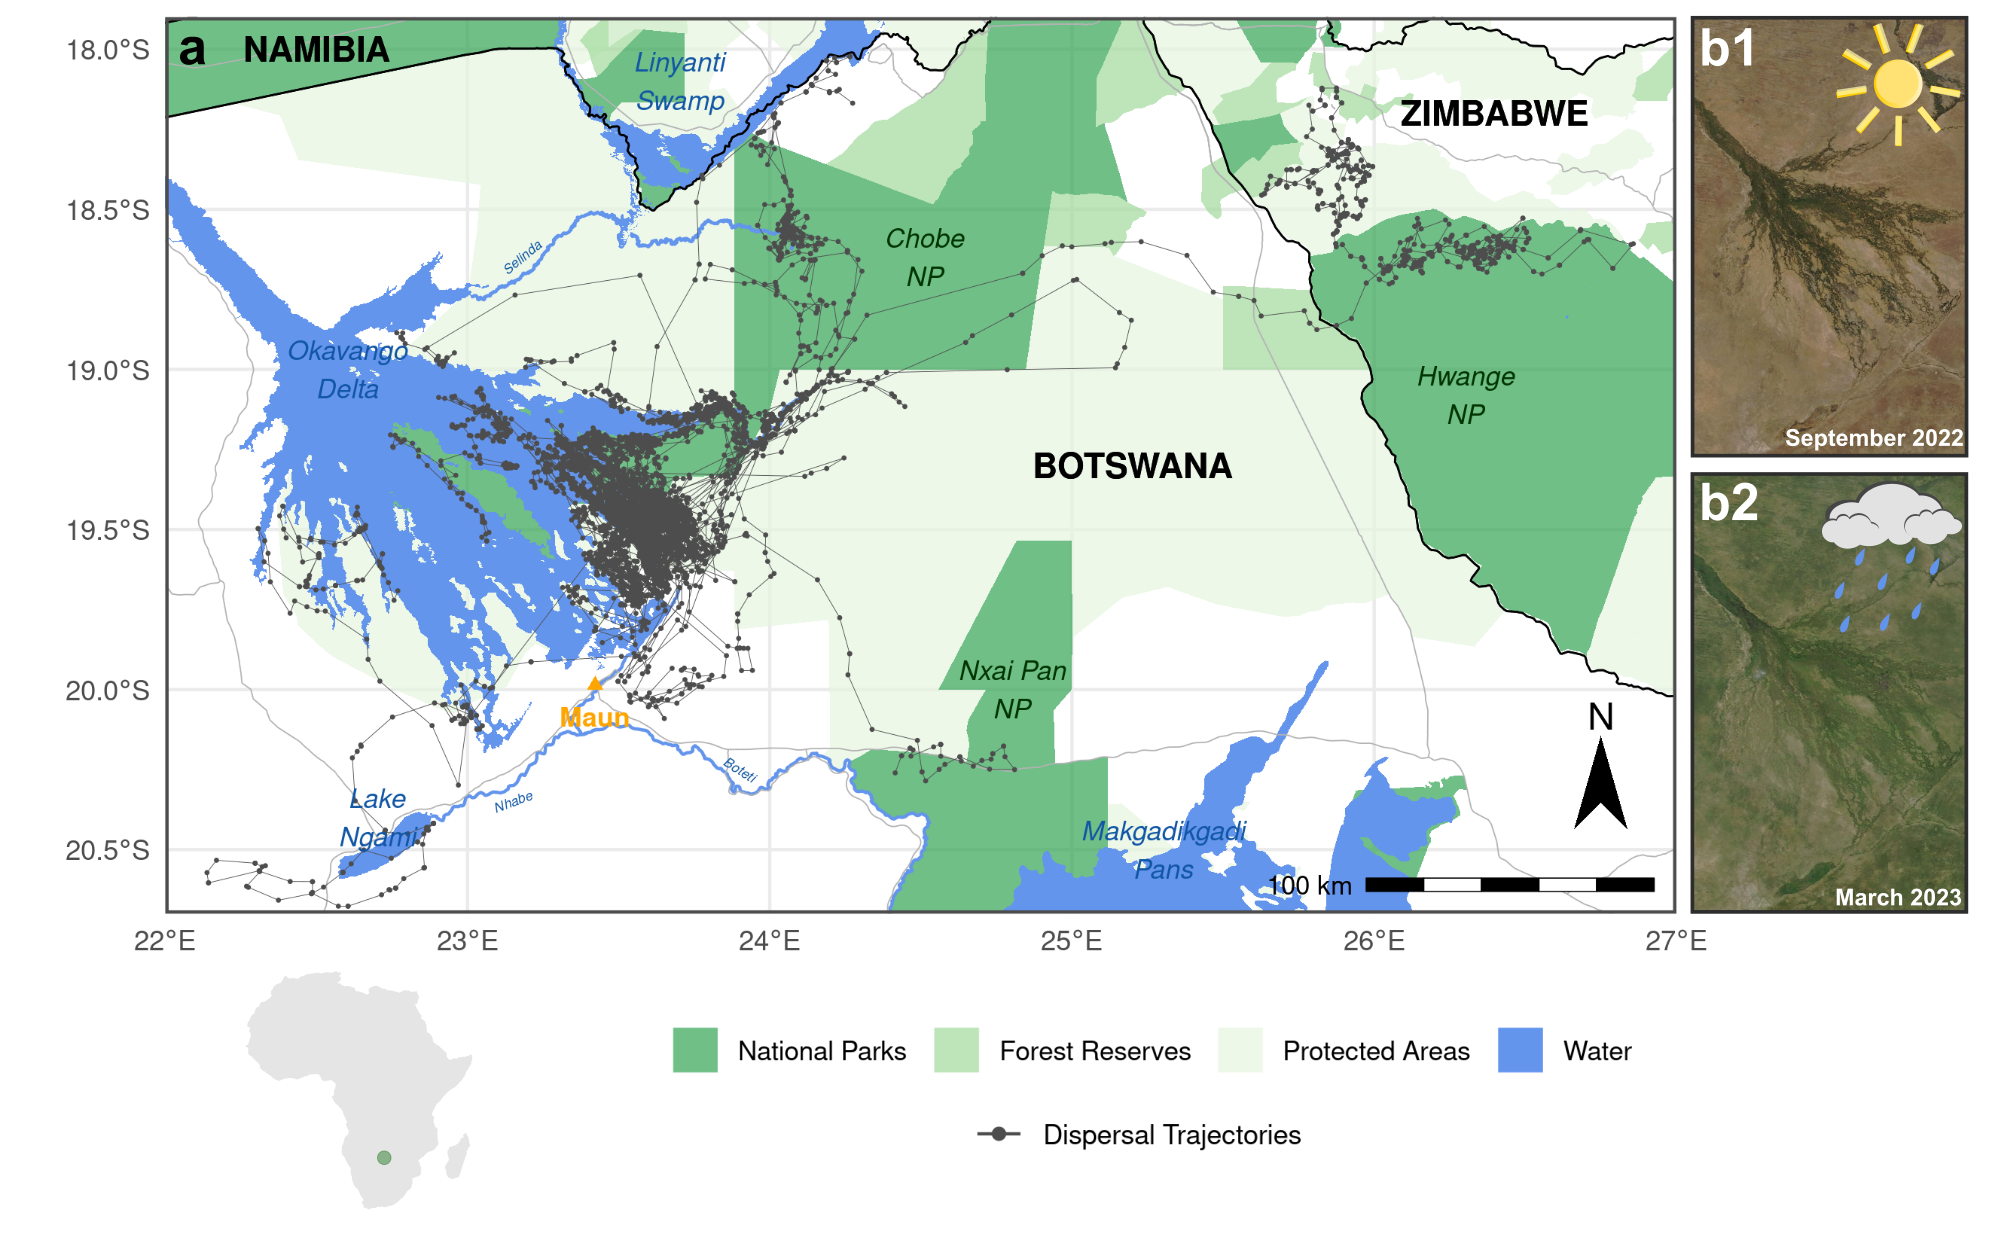
\includegraphics[width = \textwidth]{Figures/StudyArea.png} \caption{(a) Study
  area from which data on dispersing African wild dogs were collected. Dispersal
  trajectories are plotted in dark gray. The study area encompassed parts of the
  Okavango Delta in northern Botswana, a highly dynamic, flood-pulse-driven
  ecosystem. The entire study area undergoes substantial seasonal changes, as
  can be seen from two satellite images taken during peak dry season (b1) and
  peak rainy season (b2). Notably, the flood of the Okavango Delta reaches its
  maximum extent during peak dry season between August and September.}
  \label{StudyAreaCH3}
 \end{center}
\end{figure}

\begin{figure}[htpb]
\begin{center}
  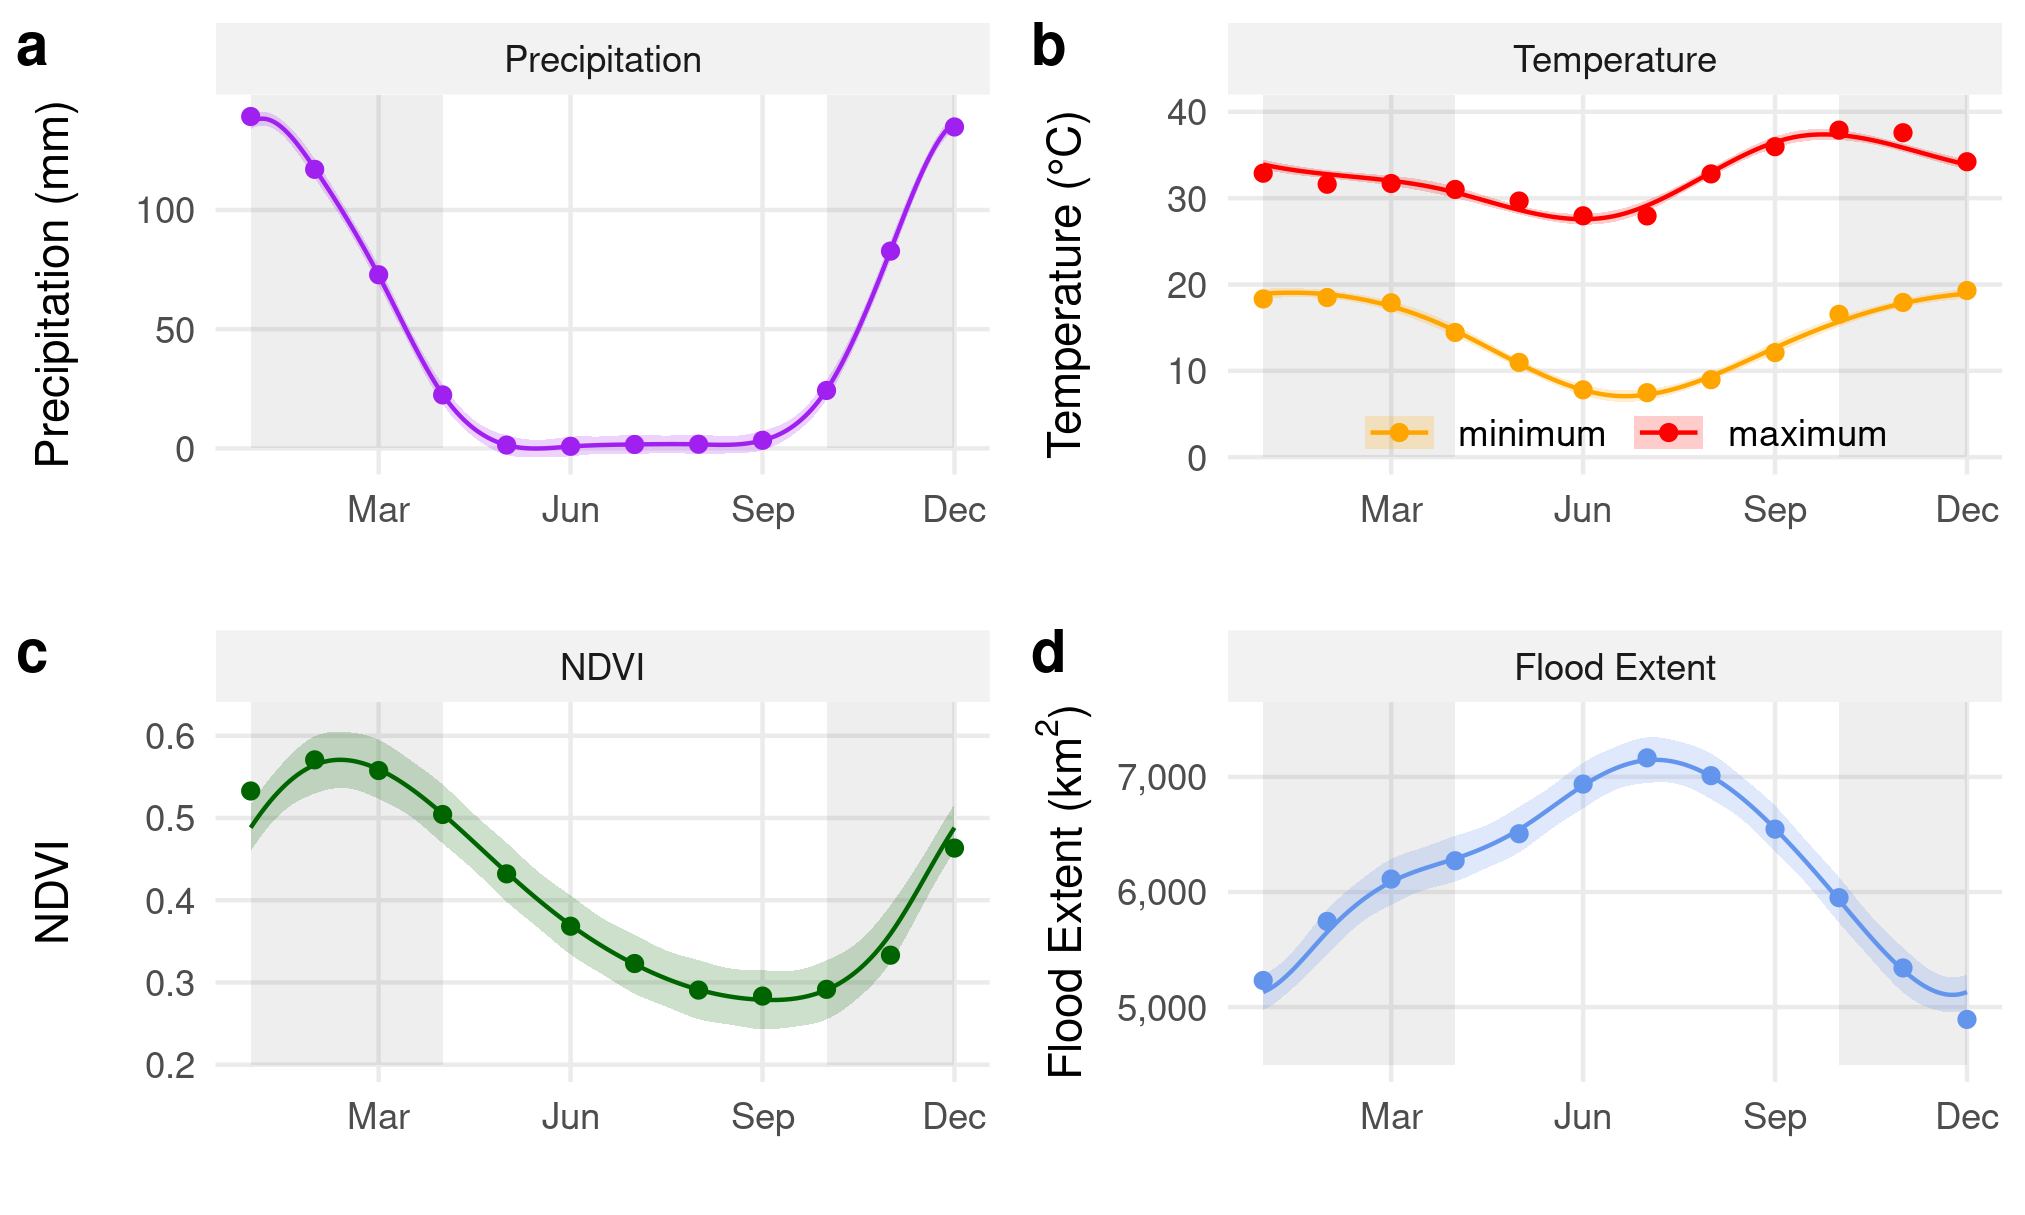
\includegraphics[width = \textwidth]{Figures/SeasonalCovariates.png}
  \caption{Illustration of how some of the covariates considered in this study
  vary across seasons. The wet season spans mid-October to mid-April (shaded in
  gray), the remainder is considered as dry season. Data for the graphs were
  obtained from (a) JAXA GSMaP, (b) ERA5, (c) MODIS MOD13Q1, and (d) remote
  sensed MOD43A4 satellite images. Smoothing curves were fitted using GAMs as
  implemented in the \texttt{mgcv} \texttt{R}-package \citep{Wood.2011}.}
  \label{Seasonality}
\end{center}
\end{figure}

\subsection{GPS Data}

Between \inputy{GeneralMetrics/GPSFromYear} and
\inputy{GeneralMetrics/GPSToYear}, we collected GPS data on
\inputy{GeneralMetrics/CollarsTotal} dispersing wild dog coalitions
(\inputy{GeneralMetrics/CollarsFemales} female coalitions,
\inputy{GeneralMetrics/CollarsMales} male coalitions; \Cref{StudyAreaCH3}b). We
programmed GPS satellite collars to record GPS locations at 01:00, 05:00, 09:00,
17:00, and 21:00. The eight-hour window between 09:00 and 17:00 can be
considered comparable to a four-hour window, as wild dogs generally rest between
11:00 and 15:00, leaving approximately four hours of activity
\citep{Hayward.2009}. The collected GPS data were regularly transmitted to a
base-station via Iridium satellite, thereby allowing dispersing individuals to
be monitored, even if they ventured across national borders. In total, we
obtained \inputy{GeneralMetrics/FixesTotal} locations during dispersal, with an
average of \inputy{GeneralMetrics/FixesMeanSD} locations per coalition.
Occasionally, the acquisition of a GPS location failed (success rate =
\inputy{GeneralMetrics/AcquisitionRate}\%), resulting in slight deviations from
the aspired four-hourly schedule. Further details on the GPS collar fitting
procedure and how we distinguished between dispersal and resident movements can
be found in \citet{Cozzi.2020} and \citet{Hofmann.2021}.

\subsection{Covariates}

We represented the physical landscape through which dispersers moved by a suite
of spatial covariate layers known to influence wild dog movements during
dispersal. We broadly categorized these spatial covariates into descriptors of
(1) landscape characteristics, (2) climatic conditions, and (3) anthropogenic
features (\Cref{CovariatesCH3}; see \citealp{Hofmann.2021, Hofmann.2023}).
Besides spatial covariates, we also prepared a series of covariates relating to
(4) light availability (\Cref{CovariatesCH3}; see Cozzi et al. 2012). To
appropriately render seasonality in each of the spatial covariates (1-3), we
downloaded them at the highest spatial and temporal resolutions available. That
is, we obtained for each spatial covariate a stack of raster layers that spanned
the entire range of dates for which we also collected GPS data on dispersing
wild dogs. Depending on the covariate, this resulted in differing spatial and
temporal resolutions (\Cref{CovariatesCH3}). Additionally, for each spatial
covariate, we also generated a static layer, representing ``average'' conditions
across the entire duration of the study. For this, we flattened each covariate
stack into a single layer, thus removing seasonality from the spatial data
entirely. For continuous covariates, we achieved this by averaging conditions
across all collected layers, whereas for categorical (binary) layers we
identified areas that were covered by the respective category in at least 50\%
of all layers. Using the same aggregation techniques, we computed covariate
stacks representative of a typical year. That is, instead of removing
seasonality by flattening across the entire range of dates, we flattened stacks
across years, thereby eliminating year-specific effects. These latter layers
were later used in the dispersal simulation, where we needed spatial layers that
depicted seasonal dynamism across a typical year. In summary, we prepared each
covariate dynamically and statically for the entire range of dates considered,
and dynamically for an average year.

\onehalfspacing
\begin{table}[htbp]
 \begin{center}
    \caption{Covariates that were used in this study, including information on
    their temporal and spatial resolutions, as well as on the avenue through
    which the respective data were accessed or downloaded. Download methods
    printed in \texttt{typewriter} font indicate the use of an
    \texttt{R}-package that is available through CRAN or GitHub.}
    \label{CovariatesCH3}
   \begin{threeparttable}
    \begin{tabular}{lcr}
      
\begin{tabular}[t]{lcccc}
\toprule
Variable & \makecell[c]{Temporal\\Resolution} & \makecell[c]{Spatial\\Resolution} & Source & \makecell[c]{Download\\Method}\\
\midrule
\addlinespace[0.3em]
\multicolumn{5}{l}{(1) Landscape Characteristics}\\
\hspace{1em}Trees & 1 year & 250 m & MODIS MOD44B & \texttt{RGISTools}\\
\hspace{1em}Shrubs / grassland & 1 year & 250 m & MODIS MOD44B & \texttt{RGISTools}\\
\hspace{1em}NDVI & 16 days & 250 m & MODIS MOD13Q1 & \texttt{rgee}\\
\cellcolor[HTML]{f2f2f2}{\hspace{1em}Rivers} & \cellcolor[HTML]{f2f2f2}{static} & \cellcolor[HTML]{f2f2f2}{90 m} & \cellcolor[HTML]{f2f2f2}{MERIT Hydro} & \cellcolor[HTML]{f2f2f2}{website}\\
\cellcolor[HTML]{f2f2f2}{\hspace{1em}Permanent water} & \cellcolor[HTML]{f2f2f2}{static} & \cellcolor[HTML]{f2f2f2}{30 m} & \cellcolor[HTML]{f2f2f2}{Globeland30} & \cellcolor[HTML]{f2f2f2}{website}\\
\cellcolor[HTML]{f2f2f2}{\hspace{1em}Floodwater} & \cellcolor[HTML]{f2f2f2}{8 days} & \cellcolor[HTML]{f2f2f2}{500 m} & \cellcolor[HTML]{f2f2f2}{MOD34A4} & \cellcolor[HTML]{f2f2f2}{\texttt{floodmapr}}\\
\hspace{1em}Distance to water & 8 days & 500 m & MOD43A4 & \texttt{floodmapr}\\
\hspace{1em}Pans & 5/10 days & 10 m & Sentinel 2 & \texttt{sen2r}\\
\hspace{1em}Distance to pans & 5/10 days & 10 m & Sentinel 2 & \texttt{sen2r}\\
\addlinespace[0.3em]
\multicolumn{5}{l}{(2) Climate Descriptors}\\
\hspace{1em}Temperature & 4 hours & 10 km & ERA5 & \texttt{rgee}\\
\hspace{1em}Precipitation & 4 hours & 10 km & JAXA GSMaP & \texttt{rgee}\\
\addlinespace[0.3em]
\multicolumn{5}{l}{(3) Anthropogenic Features}\\
\cellcolor[HTML]{f2f2f2}{\hspace{1em}Human density} & \cellcolor[HTML]{f2f2f2}{static} & \cellcolor[HTML]{f2f2f2}{30 m} & \cellcolor[HTML]{f2f2f2}{Facebook} & \cellcolor[HTML]{f2f2f2}{website}\\
\cellcolor[HTML]{f2f2f2}{\hspace{1em}Agriculture} & \cellcolor[HTML]{f2f2f2}{static} & \cellcolor[HTML]{f2f2f2}{30 m} & \cellcolor[HTML]{f2f2f2}{Globeland30 / Cropland} & \cellcolor[HTML]{f2f2f2}{website}\\
\cellcolor[HTML]{f2f2f2}{\hspace{1em}Roads} & \cellcolor[HTML]{f2f2f2}{static} & \cellcolor[HTML]{f2f2f2}{vectorized} & \cellcolor[HTML]{f2f2f2}{Open Street Map} & \cellcolor[HTML]{f2f2f2}{website}\\
\addlinespace[0.3em]
\multicolumn{5}{l}{(4) Light Availability}\\
\cellcolor[HTML]{f2f2f2}{\hspace{1em}Night} & \cellcolor[HTML]{f2f2f2}{4 hours} & \cellcolor[HTML]{f2f2f2}{-} & \cellcolor[HTML]{f2f2f2}{-} & \cellcolor[HTML]{f2f2f2}{\texttt{moonlit}}\\
\cellcolor[HTML]{f2f2f2}{\hspace{1em}Moon illumination} & \cellcolor[HTML]{f2f2f2}{4 hours} & \cellcolor[HTML]{f2f2f2}{-} & \cellcolor[HTML]{f2f2f2}{-} & \cellcolor[HTML]{f2f2f2}{\texttt{moonlit}}\\
\bottomrule
\end{tabular}

    \end{tabular}
    \begin{tablenotes}
      \item \textit{Note:} The covariates in gray were combined into proxies for
      water, human influence, and brightness, respectively. Detailed
      aggregation procedures are provided in \citet{Hofmann.2021}.
    \end{tablenotes}
   \end{threeparttable}
 \end{center}
\end{table}
\doublespacing

\subsubsection{Landscape Characteristics}

We used data from the MODIS Vegetation Continuous Fields dataset (MOD44B V061;
\citealp{DiMiceli.2022}) to represent different vegetation types across the
study area. The MOD44B dataset comprises three continuous layers, depicting the
percentage cover of woodland, shrubs/grassland, and bareland, respectively. The
three layers added up to 100\%, so we dropped bareland from further analysis,
thus preventing perfect multi-collinearity. The MOD44B product is updated on day
65 of each year, so we used the \texttt{R}-package \texttt{RGISTools}
\citep{Perez-Goya.2020} to download yearly updated layers, each at a resolution
of 250m x 250m. We also obtained information on the NDVI through the MODIS
MOD13Q1 dataset \citep{Didan.2015}, which also has a resolution of 250m x 250m.
This product is updated every 16 days, and we accessed the respective data
through Google Earth Engine \citep{Gorelick.2017} using the \texttt{R}-package
\texttt{rgee} \citep{Aybar.2024}. To depict large, permanent water-bodies, we
employed the Globeland30 dataset, from which we only retained the land-cover
class water, while setting all other categories to dryland. Similarly, we used
the MERIT Hydro dataset to obtain information on permanent rivers
\citep{Yamazaki.2019}. To dynamically render large water-bodies, particularly
the floodwaters of the Okavango Delta, we prepared weekly updated floodmaps
using remote sensed MODIS MOD43A4 satellite images. The underlying floodmapping
algorithm is described by detail by \citet{Wolski.2017} and \citet{Hofmann.2021}
and is implemented in the \texttt{floodmapr} package (available on GitHub;
\url{https://github.com/DavidDHofmann/floodmapr}). We combined the water
(static), river (static), and flood layers (dynamic) into a single stack with a
resolution of 500m x 500m (\Cref{CovariatesCH3}). Finally, we employed remote
sensing to detect small, ephemeral water bodies (i.e., pans) using a custom
random-forest classifier applied to Sentinel 2 satellite imagery
(\citealp{EuropeanSpaceAgency.2018}; details of the classifier in
\Cref{PanMappingApproach}). Sentinel 2 has a resolution of 10m and is therefore
particularly useful for obtaining information on small landscape features. Even
though Sentinel 2 satellite imagery is updated every 5 days, cloud cover often
prohibited the computation of a ``pan-map''. Consequently, we settled for
monthly updated composite images, which effectively alleviated problems due to
cloud cover. In summary, we produced one stack of layers representing major
water bodies, and another stack of layers representing ephemeral water bodies
(pans). For both, we also computed corresponding distance-to stacks, indicating
the distance to major and ephemeral water bodies, respectively.

\subsubsection{Climate Descriptors}

We obtained hourly updated spatial layers on 2m above-ground temperature from
the ERA5-Land dataset \citep{Munoz-Sabater.2021} and hourly updated
precipitation estimates from the Global Satellite Mapping of Precipitation
dataset \citep{Kubota.2020}. Both datasets were accessed and downloaded through
Google Earth Engine \citep{Gorelick.2017} using the \texttt{rgee} package
\citep{Aybar.2024} and had a resolution of 10km x 10km. To match one-hourly
temperature and precipitation estimates with the four-hourly GPS data on
dispersing wild dogs, we computed average precipitation and temperature values
over four hourly periods that matched the GPS collection schedule.

\subsubsection{Anthropogenic Features}

We combined information on human density, agricultural activities, and roads
into a single proxy, which we generically termed human influence. We sourced
information on human density from Facebook's high resolution human density
dataset \citep{Tiecke.2017}, which we downloaded from the humdata website
(\url{www.data.humdata.org}). We obtained information on the presence of
agricultural fields from the Globeland30 \citep{Chen.2015} and Cropland
\citep{Xiong.2017} datasets. We  downloaded shapefiles comprising main tar roads
from OpenStreetMaps \citep{OpenStreetMapContributors.2017}. Ultimately, we
merged all anthropogenic features into a single layer that had a resolution of
250m x 250m (details are provided by \citealp{Hofmann.2021}) .

\subsubsection{Light Availability}

We computed light availability using the \texttt{suncalc} and \texttt{moonlit}
\texttt{R}-packages \citep{Thieurmel.2022, Smielak.2023} for the central
coordinates of our study area at a 5-minute temporal resolution. The set of
light statistics comprised a binary variable separating day and night (i.e., sun
$<$ -18 \degree below the horizon) and a continuous estimate of moonlight
illumination, relative to the maximum moon illumination. Based on those
covariates, we generated a binary covariate separating bright from dark
conditions. Bright conditions encompassed all daytime hours and those nighttime
periods during which the moon was present in the sky and illuminated by
approximately one-fourth; conversely, dark conditions included nighttime periods
during which the moon was absent from the sky or present and only minimally
illuminated (further details in Appendices A2 and A3).

\subsection{Step-Selection Models}

We modeled dispersers' movement kernel and habitat selection using integrated
step-selection functions (iSSFs, \citealp{Fortin.2005, Avgar.2016}), following
the procedure described by \citet{Muff.2020}. For this, we identified bursts of
subsequent GPS locations where the duration between two GPS locations did not
exceed 4 hours (\(\pm\) 15 minutes) or 8 hours (\(\pm\) 30 minutes, for data
recorded between 09:00 and 17:00). Within each burst, we converted locations
into steps, where a step represented the straight line segment between two
consecutive locations \citep{Turchin.1998}. For each step, we computed the
associated step length (sl, in meters) and relative turning angle (ta, in
radians). After this pre-processing, a total of \inputy{GeneralMetrics/SSFTotal}
dispersing coalitions (\inputy{GeneralMetrics/SSFFemales} female coalitions,
\inputy{GeneralMetrics/SSFMales} male coalitions) remained for further analyses.
4 coalitions dropped due to temporally irregular data. The final dataset
comprised \inputy{GeneralMetrics/StepsTotal} steps
(\inputy{GeneralMetrics/StepsMeanSD} per coalition), which we further
categorized into data collected during the wet season (15 October to 15 April)
and data collected during the dry season (15 April to 15 October), yielding
\inputy{GeneralMetrics/NumberStepsDry} steps
(\inputy{GeneralMetrics/PercentageStepsDry}\%) during the dry season and
\inputy{GeneralMetrics/NumberStepsWet} steps
(\inputy{GeneralMetrics/PercentageStepsWet}\%) during the wet season.

We paired each \textit{observed} step with a set of 100 \textit{random} steps,
generated by sampling turning angles from  a uniform distribution U(\(-\pi,
+\pi\)) and step lengths from a gamma distribution fitted to observed steps
(scale \(\theta\) = \inputy{GeneralMetrics/GammaScale} and shape \(k\) =
\inputy{GeneralMetrics/GammaShape}). Together, an observed step and its
associated random steps formed a stratum that received a unique identifier.
Along each step, we extracted covariate values from the underlying spatial
layers, and we assigned the appropriate light conditions (\Cref{CovariatesCH3}).
We opted for covariate extraction \textit{along} steps rather than \textit{at
their endpoints}, as we believed that environmental conditions along steps were
relevant in determining wild dog movement. For continuous covariates, we
computed average values along each step, for categorical covariates the
percentage cover of each category along the step. To model a decreasing marginal
impact of ``distance-to'' variables, we included their square-root as predictors
in the final models. To facilitate model convergence, we normalized extracted
values to a range between zero and one.

To estimate movement and habitat parameters of interest, we applied the maximum
likelihood procedure proposed by \citet{Muff.2020}, using the \texttt{glmmTMB}
package \citep{Brooks.2017}. To examine whether the effect of accounting for
seasonality was modulated by the model structure, we employed two separate model
formulas that were both generated based on knowledge about wild dog dispersal
movements previous studies \citep{Hofmann.2021, Hofmann.2023}. In the
\textit{simple formula}, we merely included covariates relating to landscape
characteristics and anthropogenic features, alongside the movement descriptors
(sl, log(sl), and cos(ta)) that are mandatory to fit an iSSF \citep{Avgar.2017,
Fieberg.2021}. This formula is most akin to the type of formulas that are
usually used with permeability-based approaches, which lack a mechanistic
understanding of movement. In the \textit{complex formula}, by contrast, we
included several additional interactions between step-descriptors, landscape
characteristics, climate descriptors and light availability, rendering that wild
dog movement during dispersal may be affected by such interactions. In both
formulas, we also included a stratum-specific intercept with a large fixed
variance ($10^6$, \citealp{Muff.2020}), and used dispersing coalition ID to
model random slopes for all main effects. To ensure comparability among each of
the six configurations presented in our framework (\Cref{GraphicalAbstractCH3}),
we employed the same model formulas across all of them. However, we fitted
models that differed in their degree of dynamism, as highlighted in
\Cref{GraphicalAbstractCH3}a. Models one and two were fit using static
covariates, with model one being a single-season model and model two being a
multi-season model (wet vs. dry). Models three and four, by contrast, were fit
using dynamic covariates, with model three being a single-season model, and
model four being a multi-season model (wet vs. dry). Each model was once fit
using the simple formula, once using the complex formula. To quantify how many
random steps were necessary before model estimates stabilized (sensu
\citealp{Fieberg.2021}), we fitted each model with 5, 10, 25, 50, 75, and 100
random steps.

\subsection{Validation}

We compared the predictive efficacy of each of the six configurations presented
in \Cref{GraphicalAbstractCH3}b using k-fold cross-validation for case-control
studies \citep{Fortin.2009}. For this, we split the data into training and
validation sets using an 80:20 ratio and fit the four iSSF models described
above. We then used the obtained $\beta$-estimates to predict the probability of
each random and observed step in the validation set for being chosen. Depending
on the configuration, we predicted step-probabilities using static or dynamic
covariates. Within each stratum, we assigned ranks 1-101 to each step based on
predicted probabilities and recorded the number of times the observed step was
assigned each rank. Finally, we computed Spearman's rank correlation between
ranks and associated frequencies $r_{s, realized}$. The better a model's
predictive ability, the more negative $r_{s, realized}$ should be (i.e., the
less often the observed step should be assigned a low rank). For reference, we
also computed Spearman's rank correlation for randomized preferences ($r_{s,
random}$), which we achieved by removing the observed step from each stratum and
identifying the rank of a randomly chosen step. We replicated this validation
procedure 100 times and employed ANOVA to compare the predictive efficacy of
different configurations.

\subsection{Simulations}

To assess differences in predicted connectivity upon increasing seasonal
dynamism, we ran dispersal simulations under the two most distinct
configurations, i.e. the fully static (SSS, \Cref{GraphicalAbstractCH3}) and
fully dynamic (DMD, \Cref{GraphicalAbstractCH3}) configurations. As source areas
to initiate dispersers, we defined three distinct regions known to host viable
wild dog populations (\Cref{StudyAreaCH3}). The definition of these areas was
somewhat arbitrary, albeit we deliberately selected areas in the west and east
of the Okavango Delta to examine potential influences of flooding on
connectivity (sensu \citealp{Hofmann.2024}). We also selected a more
independent location (Nxai Pan; \Cref{StudyAreaCH3}) that was not influenced
directly by the Okavango Delta's flood extent. To initiate simulated dispersal
trajectories, we randomly placed 1,000 start points within each of these source
area, with start times that were equally distributed across the year. To
simulate dispersal and obtain connectivity maps under both configurations, we
applied the simulation algorithm for iSSFs described by \citet{Signer.2017} and
employed by \citet{Hofmann.2023}. A similar algorithm has recently been added to
the \texttt{amt} \texttt{R}-package \citep{Signer.2024}. We applied the
simulation algorithm as follows. Originating from the start point, we generated
a set of 25 random steps by sampling step lengths from the fitted gamma
distribution and turning angles from a uniform distribution. Along each random
step, we extracted spatial covariates, computed relevant movement metrics (sl,
log(sl), and cos(ta)), and assigned light conditions. We then employed the
fitted iSSF model to predict the probability of each step for being chosen, thus
generating a ``redistribution kernel'' around the current location of the
simulated individual \citep{Signer.2017, Signer.2024}. Based on this kernel, we
sampled one of the steps and updated the simulated individual's position and
time. We repeated the procedure until a total of 2,000 steps were realized
($\sim$ 400 dispersal days).

Depending on the configuration, we employed different spatial covariates and
preferences during the simulation. For the SSS configuration, we omitted any
seasonality, using the static set of covariates and assuming dispersers to
exhibit the same preferences (i.e., $\beta$-estimates) across seasons. For the
DMD configuration, on the other hand, we updated covariates and preferences
dynamically as the simulated individuals moved. More specifically, we generated
a new covariate stack after every simulated step, comprising spatial layers that
best represented environmental conditions at that particular point in time
(\Cref{Schematic}). For this purpose, we employed the set of covariates
representing an average year. Similarly, we predicted the redistribution kernel
using $\beta$-estimates from the appropriate season. Finally, we obtained
heatmaps (connectivity maps, utilization distributions) based on simulated
dispersal trajectories under both configurations.

\begin{figure}[htpb]
 \begin{center}
  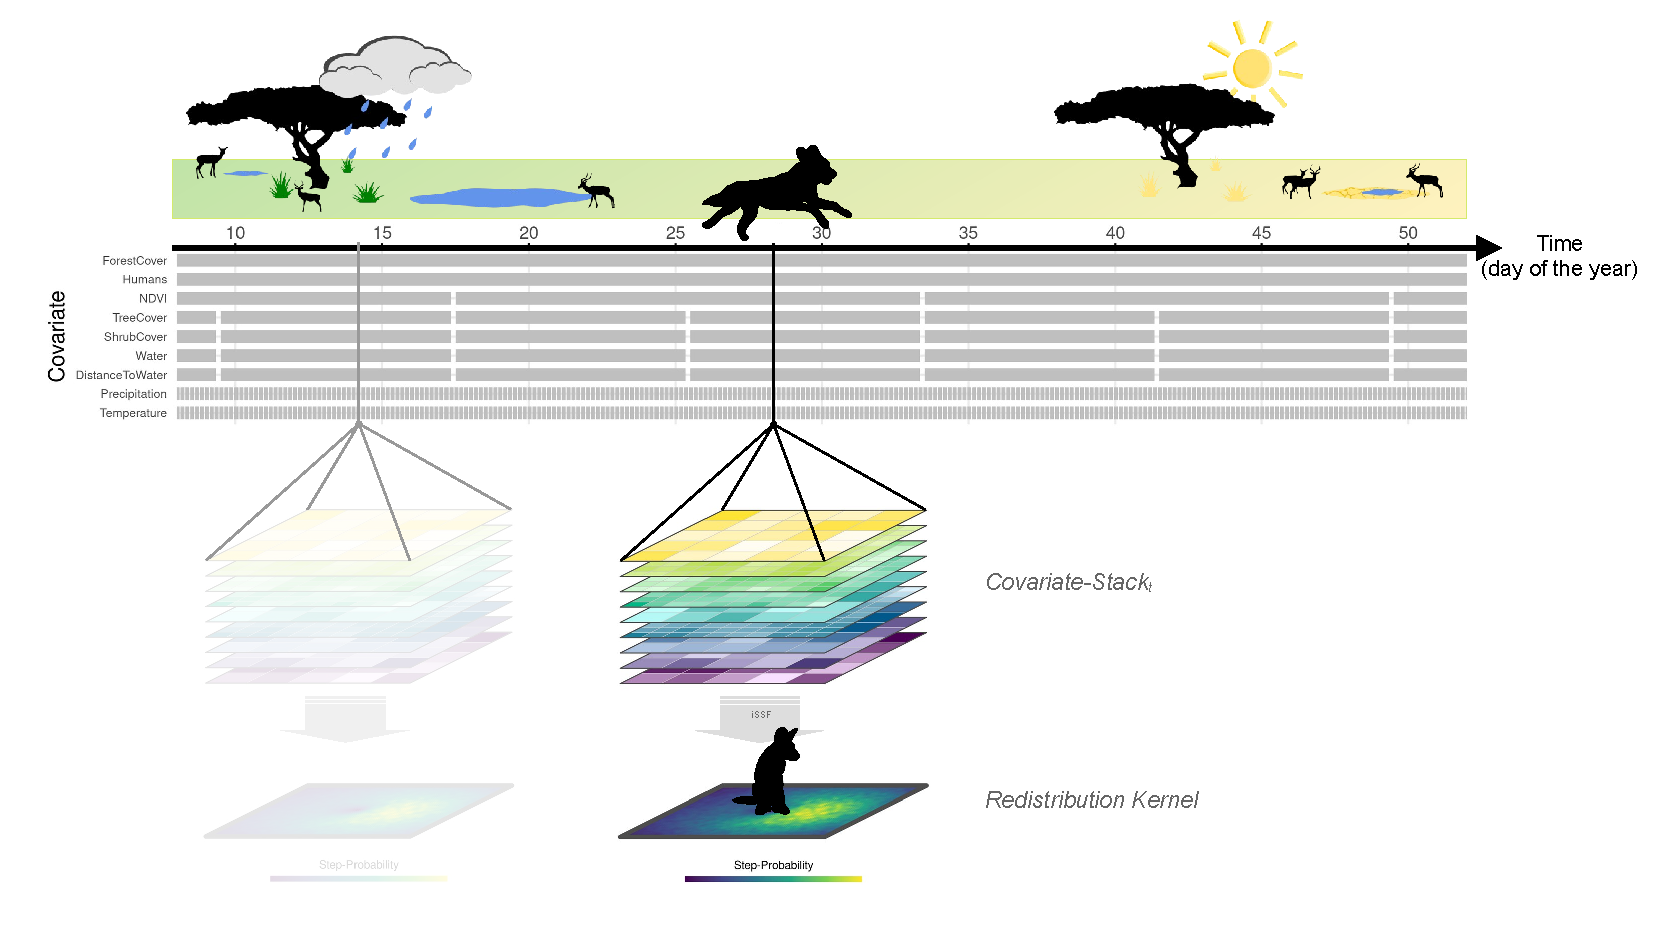
\includegraphics[width = \textwidth]{Figures/Schematic}
  \caption{Schematic illustration of our dispersal simulation with dynamic
  covariates. As the simulation proceeded, the underlying spatial covariates
  (symbolized by the stack of layers) were updated. Depending on the covariate,
  the update frequency varied from a few hours (e.g., temperature) to multiple
  months (e.g., shrub cover). Each gray block represents a single layer and the
  duration for which it was ``active''. Originating from the current position of
  the simulated animal, a new redistribution kernel was derived. We generated
  redistribution kernels by proposing a set of 25 random steps and applying the
  parametrized step-selection model to predict the probability of each step for
  being chosen. Based on this kernel, one location was randomly sampled and the
  animal's position and time updated. This procedure was then repeated until
  2,000 steps ($\sim 400$ dispersal days) were simulated.}
  \label{Schematic}
 \end{center}
\end{figure}

\section{Results}

Due to convergence issues, we removed the covariates NDVI, precipitation, and
distance to pans from all analyses. Some minor convergence issues remained and
our validation procedure failed in 59 out of 1,800 validation attempts. Since
failures occurred across different configurations and were not clustered around
one specific configuration, we deemed their exclusion of no concern.

\subsection{Step-Selection Models}

Patterns of habitat selection and movement behavior were qualitatively similar,
irrespective of whether models were fit using static or dynamic covariates
(\Cref{MovementModelCH3}, \Cref{ModelsStaticSimple}, \Cref{ModelsDynamicSimple},
\Cref{ModelsStaticFull}, \Cref{ModelsDynamicFull}) and irrespective of the
number of considered random steps (\Cref{Stability}). The most notable
quantitative difference when using static vs. dynamic covariates was that models
fitted using dynamic covariates resulted in narrower confidence intervals
(\Cref{MovementModelCH3}). Furthermore, effect sizes (i.e., $\beta$-estimates)
of models fit using static covariates were more pronounced than effect sizes
from models that were fit using dynamic covariates (\Cref{MovementModelCH3}).
Differences were most marked for $\beta_{DistanceToWater^{0.5}}$, which was
estimated $\approx -0.8$ using static covariates, but $\approx -0.3$ when using
dynamic covariates.

Differences in $\beta$-estimates between seasons were moderate and most
pronounced when models were fit using static covariates. For instance, when
models were fit using static covariates, $\beta_{Water}$ was $\approx -0.9$
during the dry season but $\approx 0.2$ during the wet season. When dynamic
covariates were used, by contrast, $\beta_{Water}$ was $\approx -0.6$ and
$\approx -0.3$, respectively. $\beta_{sl:Dark}$ was also markedly lower during
the wet season ($\approx -0.9$), compared to the dry season ($\approx -0.1$) but
this was independent of the type of covariates that were used. Plots that aid
with the interpretation of the models are provided in
\Cref{MovementModelInterpretation}.

\begin{figure}[htpb]
 \begin{center}
  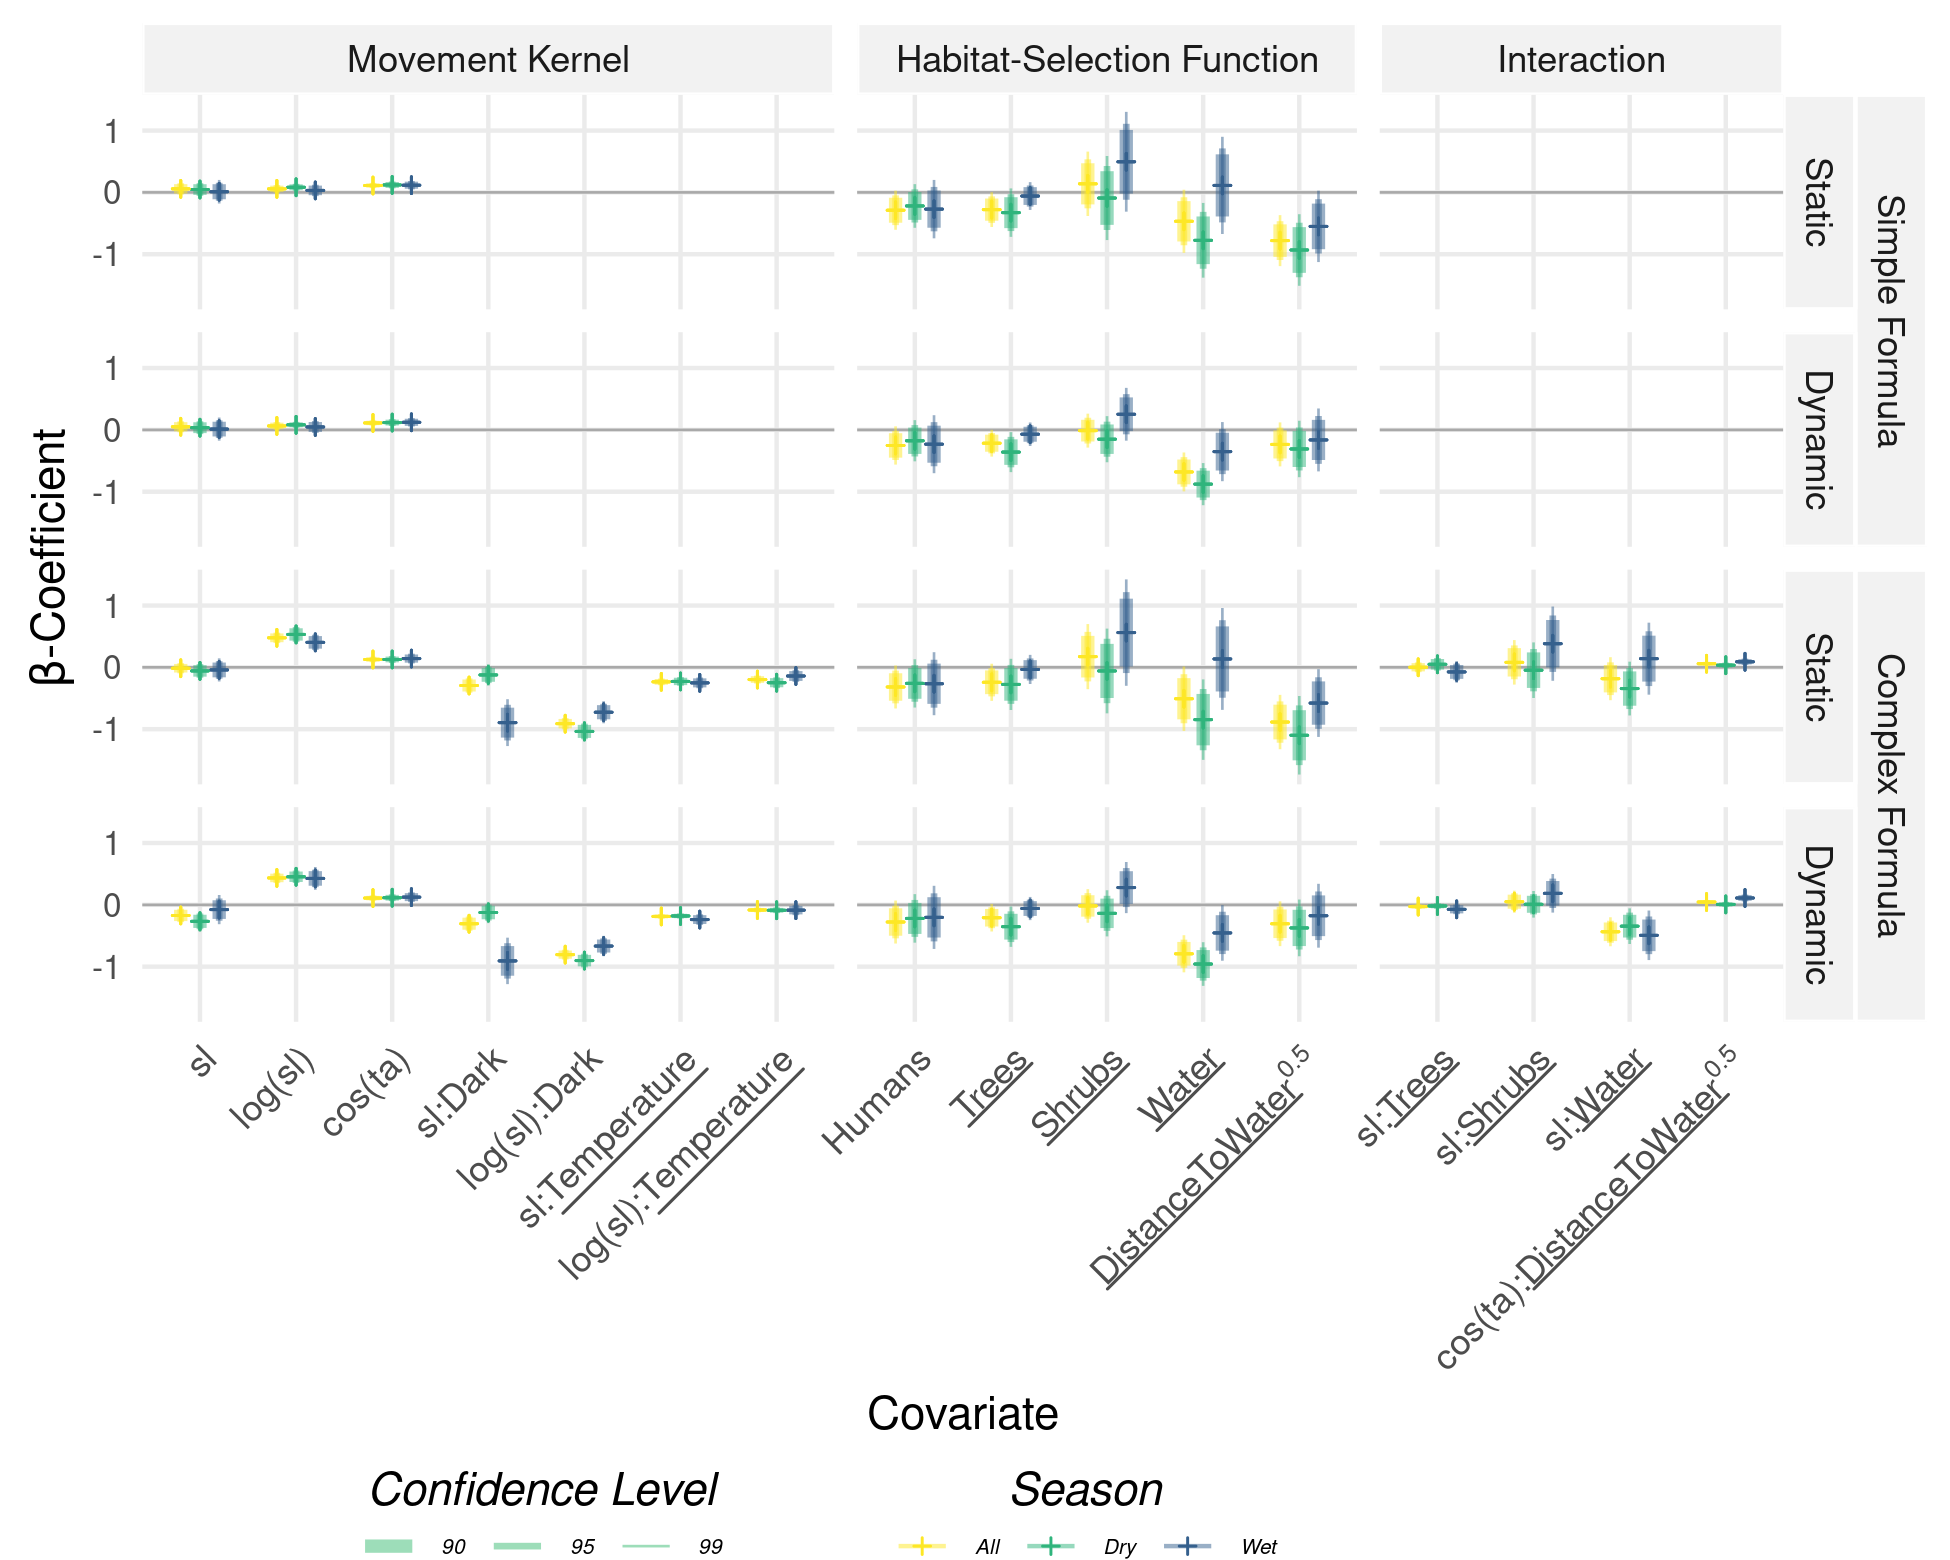
\includegraphics[width = \textwidth]{Figures/MovementModel.png}
  \caption{$\beta-$estimates from the integrated step-selection models, grouped
  by movement kernel, habitat-selection function, and their interaction. We
  either fit models using a \textit{simple formula} (without interactions) or a
  \textit{complex formula} that comprised several interaction terms that rendered
  how movement behavior depended on environmental conditions. Furthermore, we
  distinguished between models fit using \textit{static} and \textit{dynamic}
  covariates. However, only the underlined covariates differed between the
  static and dynamic configurations, as covariates were either represented as a
  single layer (static), or a stack of layers (dynamic). Furthermore, data were
  either pooled across seasons (yellow bars) or split into dry (green bars) and
  wet (blue bars) season. Results are shown for replicates that used 25 random
  steps, as all associated models converged. Note, however, that the number of
  random steps did not appear to influence model estimates (\Cref{Stability}).}
  \label{MovementModelCH3}
 \end{center}
\end{figure}

\subsection{Validation}

Spearman's rank correlation coefficients ($r$) obtained from the validation
procedure revealed that predictions using the complex formula performed markedly
better than those from the simple formula ($\bar{r}_{simple} = -0.5$,
$\bar{r}_{full} = -0.9$, \Cref{RankCorrelation}). Irrespective of the employed
model, Spearman's rank correlation differed significantly depending on the
amount of dynamism considered (simple: F(5, 593) = 26.45, p < 0.001, full: F(5,
594) = 7.14, p < 0.001), albeit with moderate effect sizes. Using the simple
formula, moving from a fully static (SSS) to a fully dynamic (DMD) configuration
decreased Spearmans's rank correlation (i.e., increased the predictive
performance) by 0.15 from -0.41 to -0.56. Using the complex formula, conversely,
moving from a fully static (SSS) to a fully dynamic (DMD) configuration even
entailed a minimal increase in $r$ (i.e., a decrease in the predictive
performance) from -0.89 to -0.88. This suggests that, our hypothesis that
increased dynamism results in better predictive performance only holds when
using the simple formula (\Cref{RankCorrelation}a), but not when employing the
complex formula (\Cref{RankCorrelation}b).

\begin{figure}[htpb]
 \begin{center}
  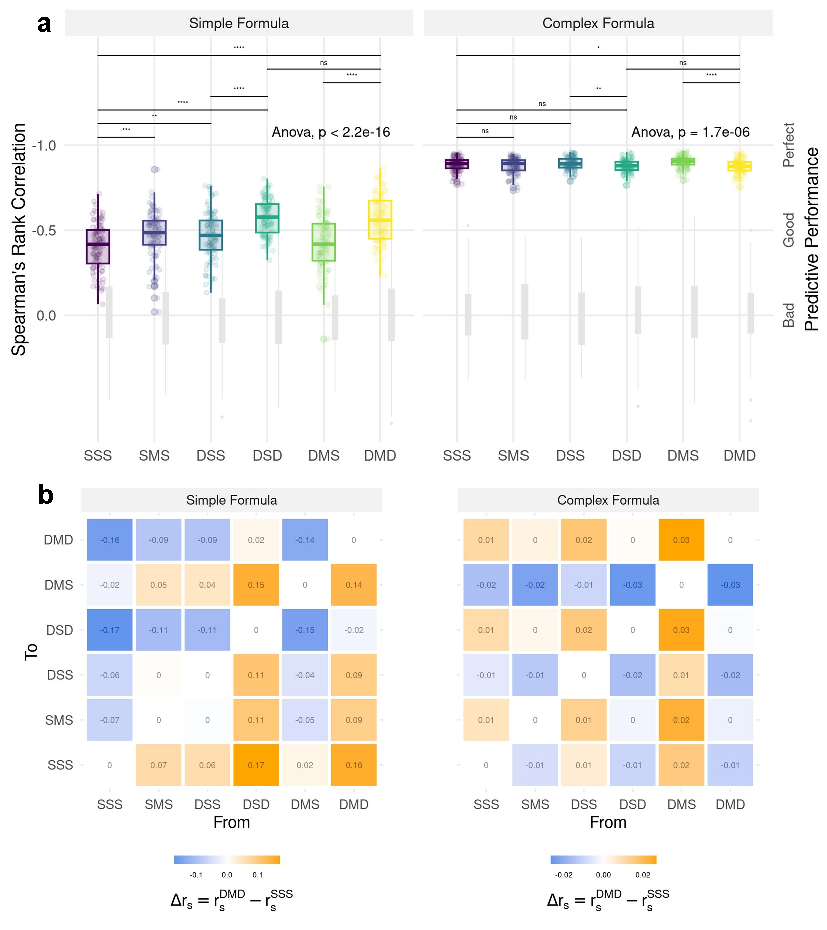
\includegraphics[width = \textwidth]{Figures/RankCorrelation.pdf}
  \caption{(a) Spearman's rank correlation across different configurations of
  dynamism that range from entirely static (SSS) to fully dynamic (DMD). The
  more negative Spearman's rank correlation, the better is the predictive
  performance under the respective configuration. Correlations were computed for
  100 replicates. Note that the y-axis is inverted to match our expectation of
  increasing performance as dynamism increases. The boxplots in light gray
  represent Spearman's rank correlation coefficients under a null model and
  serve for comparison. (b) Difference in Spearman's rank correlation when
  moving from one configuration to another. Values $< 0$ (blue) indicate an
  increase in predictive performance, whereas values $> 0$ (orange) indicate a
  decrease in predictive performance.}
  \label{RankCorrelation}
 \end{center}
\end{figure}

\subsection{Simulations}

Simulations under the most static (SSS) and dynamic (DMD) configurations
revealed different connectivity patterns (\Cref{HeatmapComparison}). In the
static configuration, simulated dispersal trajectories were more concentrated,
suggesting frequent movement across a few key habitats. In the dynamic
configuration, by contrast, simulated trajectories were more homogeneously
distributed, suggesting that movement was less restricted. When qualitatively
comparing the heatmaps generated under the simple and complex formulas,
differences are imperceptible. Given the similarities in habitat selection
emerging under the two models, this was to be expected.

\begin{figure}[htpb]
 \begin{center}
  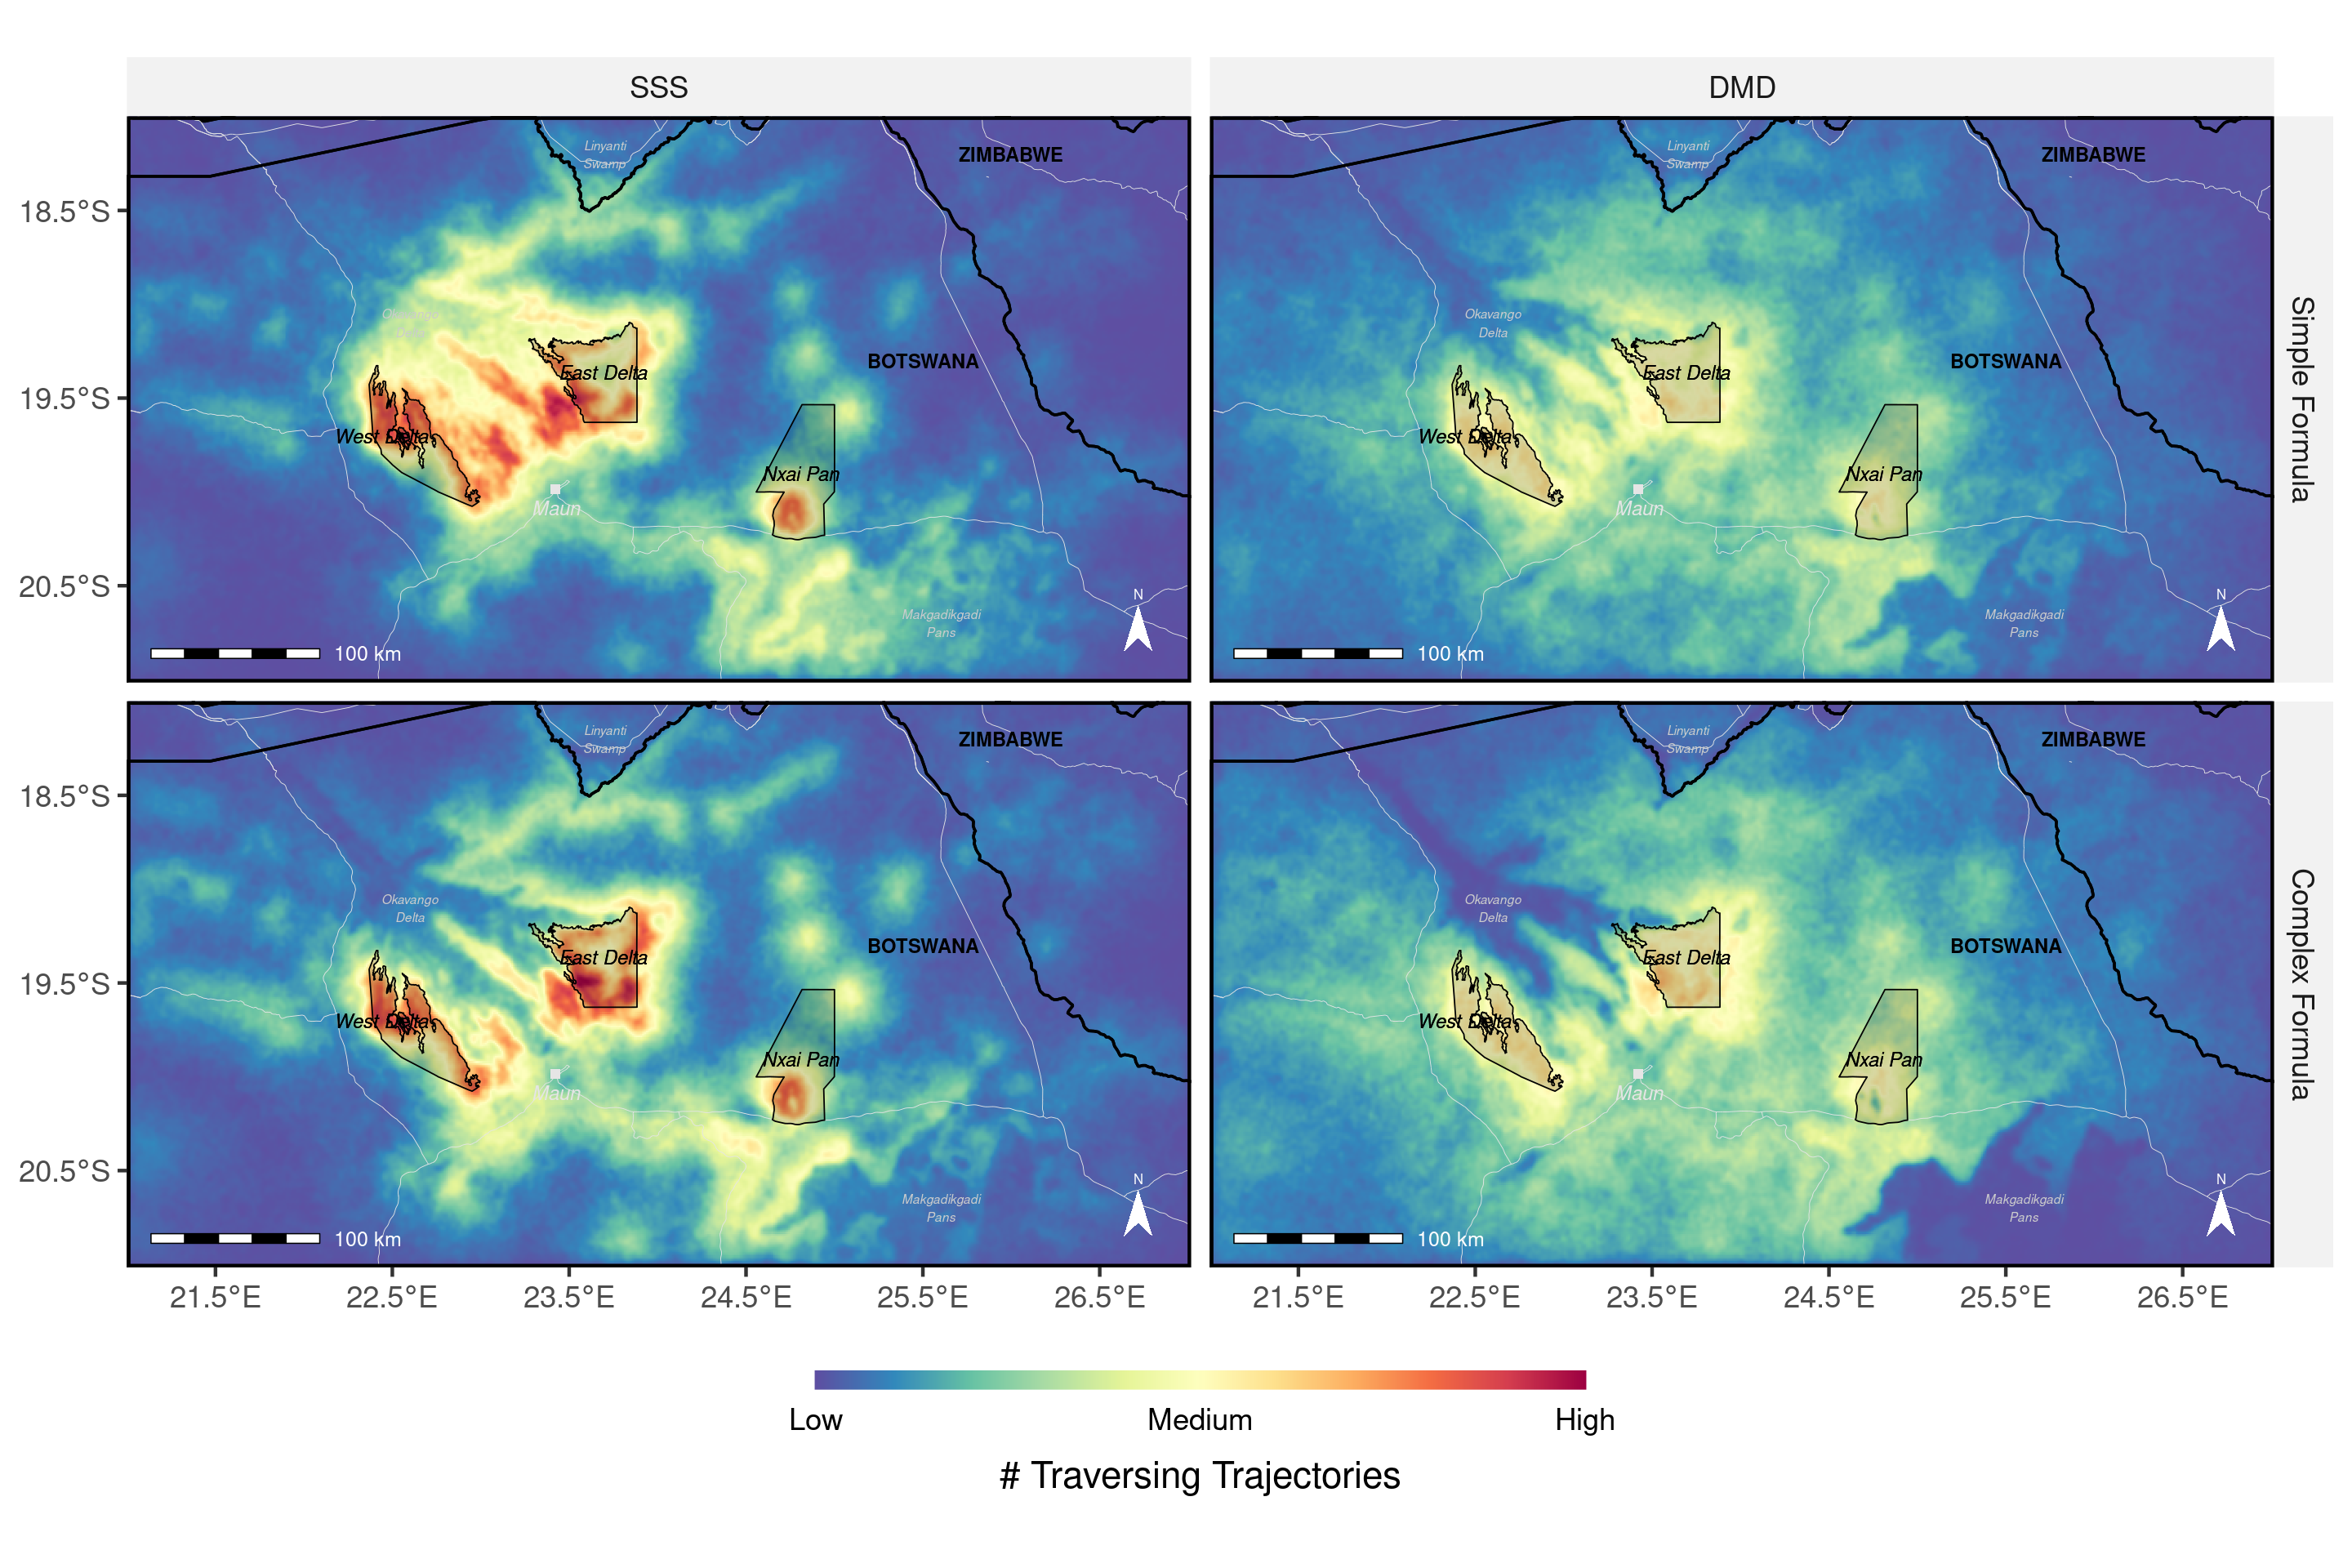
\includegraphics[width = \textwidth]{Figures/HeatmapComparison}
  \caption{Heatmaps derived under the most static (SSS) and dynamic (DMD)
  configurations. Results are shown for simulations using the simple and complex
  model formulas.}
  \label{HeatmapComparison}
 \end{center}
\end{figure}

\section{Discussion}

% \subsection{Brief Summary}

We introduced a framework to highlight that seasonality can enter a connectivity
analysis at three distinct stages; (1) when extracting spatial covariates for
fitting the selection model, (2) when fitting the selection model, and (3) when
predicting from the fitted model. Through combination, this yields six
configurations that differ in their degree of dynamism and, arguably, realism.
We fit the models associated with each configuration using GPS data on
dispersing wild dogs and employed a rigorous validation procedure to investigate
potential gains in predictive performance that can be reaped by incorporating
different levels of seasonal dynamism. Results from the fitted models showed
that including seasonality only marginally affected the inferred patterns of
habitat selection and movement behavior. Similarly, the validation procedure
suggested only moderate improvements in predictive performance upon increasing
the degree of seasonal dynamism. Crucially, these benefits were limited to an
overly simplistic model formula and vanished upon fitting a more complex one. We
therefore could not pinpoint a specific stage at which including seasonality was
particularly beneficial. Despite this, we found that dispersal simulations under
the most static and most dynamic configurations resulted in differing
connectivity patterns. Under the most static configuration, landscape
connectivity was clumped around a few hot spots, whereas it was homogeneously
distributed across the landscape under the most dynamic configuration. Finally,
our work demonstrated that simulations from IBMMs effectively allow rendering
seasonal changes in the landscape, achieving a degree of seasonal dynamism and
realism that cannot be reached using permeability-based connectivity models.

% \subsection{Moderate Improvements upon Increasing Dynamism}

Our validation procedure revealed only moderate improvements in our ability to
predict dispersal movements when increasing the degree of seasonal dynamism.
Given the system's extreme seasonal variability, this was somewhat surprising.
We believe that the absence of a more pronounced improvement can be traced back
to multiple factors. Firstly, we focused our analysis on dispersing individuals,
which cover large distances in search of potential mates and a suitable
territory \citep{McNutt.1996, Cozzi.2020}. In our case, the average 4-hourly
step length was 2.5 km, suggesting that dispersers cross and sample numerous
unfamiliar areas and potentially unsuitable habitats within short time. We thus
hypothesize that the spatial scale at which seasonality affects environmental
characteristics does not suffice to match the spatial scale at which our focal
species perceives and moves across the landscape during dispersal. A Further
explanation could be that dispersing individuals prioritize finding unoccupied
territories or areas with low competition, rather than focusing on specific
habitat types (e.g., \citealp{Creel.1996, Creel.2001}). Dispersers' habitat
selection may therefore be more strongly influenced by territorial
considerations (sensu \citealp{Cozzi.2018}) and only little affected by
seasonally changing landscape characteristics. This would also explain the
relatively weak selection or avoidance of environmental characteristics
exhibited in \Cref{MovementModelCH3}. Finally, the AWD is a generalist species
that can occupy a broad variety of habitats \citep{Woodroffe.2011}. A certain
tolerance towards changing environmental conditions can therefore be expected
and may explain why seasonal differences were faint. This holds particularly
true for dispersers, which are usually more tolerant towards unfavorable habitat
conditions as they spend little time within the same area \citep{ONeill.2020}.

% \subsection{Substantial Improvements upon Fitting a Complex Model}

In comparison to the improvements achieved by increasing dynamism, a more
significant improvement in predictive ability was achieved by moving from the
simple to the complex model formula. When employing the complex formula, we
included several interactions that accounted for the African wild dog's biology,
such as reduced movement during dark nights \citep{Cozzi.2013} or during times
of high ambient temperature \citep{Rabaiotti.2021}. We also allowed for
potential changes in dispersers' movement behavior depending on habitat
conditions, such as shorter steps in areas covered by water
\citep{Hofmann.2023}. The ability of encapsulating such a detailed and
mechanistic understanding of dispersal movements is unique to IBMMs and cannot
be achieved using permeability-based connectivity models. Even though the
additional interactions were not directly linked to connectivity, they accounted
for a substantial amount of variation in observed dispersal movements and
facilitated predictions from the fitted model. Notably, the inclusion of these
interactions elevated the predictive ability of our dispersal model to such a
high level that considering seasonal dynamism did not provide any further
improvements, irrespective of the stage at which it was considered.


% \subsection{Dynamic Connectivity}

When comparing connectivity under the most static (SSS) and dynamic (DMD)
configurations, we observed that connectivity was clumped along a few major
dispersal hotspots under the static configuration, but homogeneously distributed
across the entire landscape under the dynamic configuration. This corroborates
previous research showing that static representations tend to result in an
underestimation of connectivity because seasonal stepping stones or corridors
are missed \citep{Martensen.2017}. With the help of such seasonally-available
dispersal habitats, areas that would otherwise be difficult to reach become
accessible, even if only for a limited time. In our study, such stepping stones
could arise in two ways. Firstly, the landscape changed seasonally, which caused
spatial shifts in preferred and avoided habitats, leading to the emergence of
alternative movement corridors. In addition, habitat or movement preferences of
simulated individuals changed, which resulted in different habitat
characteristics being traversed depending on the season. In combination,
temporally varying landscape conditions and seasonally altered species
preferences resulted in a more balanced mosaic of connectivity across the year.
Importantly, the fact that connectivity was more evenly distributed across the
year does not exclude the possibility that certain areas experienced lower
connectivity seasonally. As already shown by \citet{Osipova.2019}, a static
representation may result in both an over- and under-estimation of short-term
connectivity, depending on the area and season. For conservation planning, this
implies a need to protect landscapes at broader scales, as areas that provide
little connectivity during some season may become critical during others. A
dynamic take at connectivity therefore improves our understanding of ecological
processes in dynamic landscapes and may help to identify otherwise overlooked
dispersal hotspots.

% \subsection{The Costs of Incorporating Dynamism}

Increasing seasonal dynamism to model dynamic connectivity comes at significant
costs, both in terms of data requirements and computational challenges. To
represent seasonal changes across the landscape, one needs to download and
process frequently updated spatial layers for each seasonal covariate. This is
time-consuming and implies a substantial increase in the data-volume that needs
to be handled. Because seasonal products are comparably rare, modeling dynamic
connectivity also entails a significant reduction in the number of potential
covariates and may require custom remote sensing algorithms (e.g.,
\Cref{PanMappingApproach}). Seasonal and remote sensed layers are also more
susceptible to noise and missing values, particularly during seasons when cloud
cover is frequent. Extracting covariates from seasonal layers poses a further
challenge, as covariate data can no longer be extracted from single layers, but
need to be extracted from exactly those layers that best represent environmental
conditions at the time of the respective observed or random step. This applies
to the extraction of data for model fitting, as well as when extracting data
during the simulation. Finally, splitting species data by season to parametrize
seasonal selection models can significantly reduce the amount of data remaining
per season, potentially causing convergence issues. In our case, the moderate
improvement in predictive ability did not warrant these additional efforts and
complications. This conclusion is, however, likely highly specific to our study
system. We therefore do not wish to discourage future studies from accounting
for seasonality when assessing connectivity. Instead, we would like to view our
study as an example that the benefits of increased realism do not necessarily
justify the additional complexity they bring about and that the associated costs
and benefits need to be carefully pondered \citep{Puy.2022}.

% \subsection{Validation Procedure}

Our validation procedure was focused on validation at the step level, but did
not directly test how well predictions of functional connectivity agreed with
true connectivity. This was owed to a conceptual limitation when trying to
validate seasonal connectivity as predicted from an IBMM. In seasonal
landscapes, connectivity not only varies spatially, but also temporally. A
meaningful validation therefore requires that connectivity is predicted
separately for each timestamp in the validation data. In our case, for instance,
the fact that the landscape changed every four hours (i.e., with every step)
entails that a new connectivity map would need to be developed around each
validation step. This is equivalent to generating and validating the
redistribution kernel, and therefore equivalent to validating predictions at the
step level. For this reason, we deemed the application of k-fold
cross-validation for case and control studies using Spearman's rank correlation
as an appropriate validation technique. Note, however, that Spearman's rank
correlation coefficient is heavily dependent on the number of steps per stratum
and should not be used to compare predictive efficacy across studies
(\Cref{RankCorrelationNumberSteps}). For static connectivity analyses,
alternative validation techniques exist. \citet{McClure.2016}, for instance,
proposed a suite of validation metrics (applied in \citealp{Zeller.2018} and
\citealp{Finerty.2023}) that largely work by comparing connectivity at random
locations with connectivity at locations where the focal species was observed.
Because these metrics fail to account for potential autocorrelation in the
validation data (which is usually present in GPS data), \citet{Brennan.2020}
suggested validating connectivity by applying a path- or step-selection model to
withheld data, using the connectivity map as the only spatial covariate. If the
fitted model proves significant selection towards areas of high connectivity,
predictions are indeed indicative of functional connectivity (sensu
\citealp{Brennan.2020}). Developing similar approaches for dynamic connectivity
analyses remains a task for future studies.

% \subsection{Seasonal Habitat Selection}

% In the Okavango Delta, water is among the most temporally variable landscape
% features that drives the distribution of species over large spatial scales
% \citep{McCarthy.1998, Ramberg.2006, Bartlam-Brooks.2011, Bennitt.2014}. Wild
% dogs, like most other large carnivores, may avoid a large distance to water
% because of prey-availability in its vicinity \citep{Redfern.2003, Bonyongo.2005,
% Valeix.2010}. At the same time, wild dogs are terrestrial mammals and avoid
% crossing water \citep{Cozzi.2013}, even during dispersal \citep{Hofmann.2021}.

When we fit models assuming static covariates, wild dogs displayed a preference
for areas close to water, irrespective of the season. However, water itself
appeared only to be avoided during the dry season. This was likely caused by a
misrepresentation of areas covered by water in the static configuration. Since
rainwater collected in Angola only slowly descends through the Okavango Delta's
tributaries \citep{McCarthy.1997}, large portions of the Delta's floodplains
remain dry during the wet season \citep{McCarthy.2003}. On static covariates,
which represent average conditions across both seasons, it may appear as if
individuals moved through areas covered by water, albeit in reality they likely
moved along them. Indeed, upon accounting for such seasonal changes by
considering seasonally updated covariate layers, parameter estimates from the
selection models assimilated and consistently suggested avoidance of water
across both seasons. Accounting for seasonality can therefore result in vastly
different biological insights. In this regard, our choice of splitting data into
wet and dry season based on a fixed set of dates can be viewed as limitation, as
it assumed an immediate switch from one season to another. In reality,
season-transitions are not abrupt but rather gradual and their timing may vary
from year to year. A more robust approach would therefore be to define the start
and end of each season based on bio-climatic descriptors and to ignore data
collected during transitional periods. This may imply a loss of data, but could
help to detect seasonal selection patterns. In our case, retaining all data was
necessary to ensure model convergence, but may have resulted in a
cross-contamination between seasons and therefore reduced our ability to pick up
seasonal differences estimated parameters. Indeed, other studies report that
habitat selection of their focal species varied greatly between seasons (but see
\citealp{Squires.2013}). \citet{Benz.2016}, for instance, found that dispersing
in elk (\textit{Cervus elaphus}) exhibit vastly different habitat preferences
during winter and summer. Similarly, \citet{Osipova.2019} report that habitat
selection of African elephants (\textit{Loxodonta africana}) in South Africa
differs between the wet and dry season. The importance of seasonality thus
appears to be highly system dependent.

% In cases where animals move along borders of two types of habitats
% that shift seasonally, a seasonal representation of habitat conditions seems
% paramount to prevent misleading conclusions.

% Other studies, however, report consistent preferences, irrespective of the
% season. \citet{Squires.2013}, for instance, show that habitat selection by lynx
% (\textit{Lynx lynx}) only differs little between winter and summer. Notably, the
% authors find that inferred patterns of connectivity were similar across seasons.
% However, few of them accounted for seasonality in their covariates, so it is not
% clear whether differences were are truly indicative of a behavioral changes or
% simply reflect changes in environmental conditions.

% \subsection{Conclusion}

In conclusion, we explored the importance of incorporating different degrees of
seasonal dynamism when studying dispersal and connectivity. Overall, our
findings suggested only moderate improvements in predictive performance upon
increasing the level of dynamism. Nevertheless, we found that connectivity
patterns as inferred from simulated dispersal trajectories differed vastly, with
connectivity being more evenly distributed when seasonality was accounted for.
While increased realism via improved representation of seasonal dynamism may
offer novel insights into ecological processes, its benefits must be carefully
weighed against the added complexity introduced by seasonal data and seasonal
preferences. Moving forward, our study serves as an example that while
accounting for seasonality could be crucial for some study systems, it may not
always justify the additional complexity, emphasizing the need for thoughtful
consideration of costs and benefits in future research.

% \section{Authors' Contributions}
%
% D.D.H. and G.C. conceived the study and designed methodology; D.D.H., G.C.,
% D.M.B, and J.W.M. collected the data; D.D.H. analysed the data; G.C. assisted
% with modeling; D.D.H. and G.C. wrote the first draft of the manuscript and all
% authors contributed to the drafts at several stages and gave final approval for
% publication.
%
% \section{Data Availability}
%
% Access to R-scripts to replicate our analyses will be provided through an online
% repository at the time of publication.
%
% \section{Acknowledgments \& Funding}
%
% We thank the Ministry of Environment and Tourism and the Department of Wildlife
% and National Parks of Botswana for granting permission to conduct this
% research. D.D.H. was funded by a Swiss National Science Foundation Grant No.
% 310030\_204478 to G.C.

\ifSubfilesClassLoaded{%
  \newpage
  \begin{singlespacing}
  \ifthenelse{\boolean{usebiblatex}}{
    \begin{refcontext}[sorting=nyt]
    \printbibliography
    \end{refcontext}
  } {
    \bibliography{../LiteratureBibtex}%
  }
\end{singlespacing}
}{}

\end{document}
